% Options for packages loaded elsewhere
\PassOptionsToPackage{unicode}{hyperref}
\PassOptionsToPackage{hyphens}{url}
%
\documentclass[
]{article}
\usepackage{amsmath,amssymb}
\usepackage{lmodern}
\usepackage{ifxetex,ifluatex}
\ifnum 0\ifxetex 1\fi\ifluatex 1\fi=0 % if pdftex
  \usepackage[T1]{fontenc}
  \usepackage[utf8]{inputenc}
  \usepackage{textcomp} % provide euro and other symbols
\else % if luatex or xetex
  \usepackage{unicode-math}
  \defaultfontfeatures{Scale=MatchLowercase}
  \defaultfontfeatures[\rmfamily]{Ligatures=TeX,Scale=1}
  \setmainfont[]{Arial}
\fi
% Use upquote if available, for straight quotes in verbatim environments
\IfFileExists{upquote.sty}{\usepackage{upquote}}{}
\IfFileExists{microtype.sty}{% use microtype if available
  \usepackage[]{microtype}
  \UseMicrotypeSet[protrusion]{basicmath} % disable protrusion for tt fonts
}{}
\makeatletter
\@ifundefined{KOMAClassName}{% if non-KOMA class
  \IfFileExists{parskip.sty}{%
    \usepackage{parskip}
  }{% else
    \setlength{\parindent}{0pt}
    \setlength{\parskip}{6pt plus 2pt minus 1pt}}
}{% if KOMA class
  \KOMAoptions{parskip=half}}
\makeatother
\usepackage{xcolor}
\IfFileExists{xurl.sty}{\usepackage{xurl}}{} % add URL line breaks if available
\IfFileExists{bookmark.sty}{\usepackage{bookmark}}{\usepackage{hyperref}}
\hypersetup{
  pdftitle={La raport intermédiaire},
  pdfauthor={Antoine Viguié, Aymane Berriane, Christian Alvarez Leon, Meng Wang, Yu PENG},
  hidelinks,
  pdfcreator={LaTeX via pandoc}}
\urlstyle{same} % disable monospaced font for URLs
\usepackage[margin=1in]{geometry}



\usepackage{color}
\usepackage{fancyvrb}
\newcommand{\VerbBar}{|}
\newcommand{\VERB}{\Verb[commandchars=\\\{\}]}
\DefineVerbatimEnvironment{Highlighting}{Verbatim}{commandchars=\\\{\}}
% Add ',fontsize=\small' for more characters per line
\usepackage{framed}
\definecolor{shadecolor}{RGB}{248,248,248}
\newenvironment{Shaded}{\begin{snugshade}}{\end{snugshade}}
\newcommand{\AlertTok}[1]{\textcolor[rgb]{0.94,0.16,0.16}{#1}}
\newcommand{\AnnotationTok}[1]{\textcolor[rgb]{0.56,0.35,0.01}{\textbf{\textit{#1}}}}
\newcommand{\AttributeTok}[1]{\textcolor[rgb]{0.77,0.63,0.00}{#1}}
\newcommand{\BaseNTok}[1]{\textcolor[rgb]{0.00,0.00,0.81}{#1}}
\newcommand{\BuiltInTok}[1]{#1}
\newcommand{\CharTok}[1]{\textcolor[rgb]{0.31,0.60,0.02}{#1}}
\newcommand{\CommentTok}[1]{\textcolor[rgb]{0.56,0.35,0.01}{\textit{#1}}}
\newcommand{\CommentVarTok}[1]{\textcolor[rgb]{0.56,0.35,0.01}{\textbf{\textit{#1}}}}
\newcommand{\ConstantTok}[1]{\textcolor[rgb]{0.00,0.00,0.00}{#1}}
\newcommand{\ControlFlowTok}[1]{\textcolor[rgb]{0.13,0.29,0.53}{\textbf{#1}}}
\newcommand{\DataTypeTok}[1]{\textcolor[rgb]{0.13,0.29,0.53}{#1}}
\newcommand{\DecValTok}[1]{\textcolor[rgb]{0.00,0.00,0.81}{#1}}
\newcommand{\DocumentationTok}[1]{\textcolor[rgb]{0.56,0.35,0.01}{\textbf{\textit{#1}}}}
\newcommand{\ErrorTok}[1]{\textcolor[rgb]{0.64,0.00,0.00}{\textbf{#1}}}
\newcommand{\ExtensionTok}[1]{#1}
\newcommand{\FloatTok}[1]{\textcolor[rgb]{0.00,0.00,0.81}{#1}}
\newcommand{\FunctionTok}[1]{\textcolor[rgb]{0.00,0.00,0.00}{#1}}
\newcommand{\ImportTok}[1]{#1}
\newcommand{\InformationTok}[1]{\textcolor[rgb]{0.56,0.35,0.01}{\textbf{\textit{#1}}}}
\newcommand{\KeywordTok}[1]{\textcolor[rgb]{0.13,0.29,0.53}{\textbf{#1}}}
\newcommand{\NormalTok}[1]{#1}
\newcommand{\OperatorTok}[1]{\textcolor[rgb]{0.81,0.36,0.00}{\textbf{#1}}}
\newcommand{\OtherTok}[1]{\textcolor[rgb]{0.56,0.35,0.01}{#1}}
\newcommand{\PreprocessorTok}[1]{\textcolor[rgb]{0.56,0.35,0.01}{\textit{#1}}}
\newcommand{\RegionMarkerTok}[1]{#1}
\newcommand{\SpecialCharTok}[1]{\textcolor[rgb]{0.00,0.00,0.00}{#1}}
\newcommand{\SpecialStringTok}[1]{\textcolor[rgb]{0.31,0.60,0.02}{#1}}
\newcommand{\StringTok}[1]{\textcolor[rgb]{0.31,0.60,0.02}{#1}}
\newcommand{\VariableTok}[1]{\textcolor[rgb]{0.00,0.00,0.00}{#1}}
\newcommand{\VerbatimStringTok}[1]{\textcolor[rgb]{0.31,0.60,0.02}{#1}}
\newcommand{\WarningTok}[1]{\textcolor[rgb]{0.56,0.35,0.01}{\textbf{\textit{#1}}}}
\usepackage{longtable,booktabs,array}
\usepackage{calc} % for calculating minipage widths
% Correct order of tables after \paragraph or \subparagraph
\usepackage{etoolbox}
\makeatletter
\patchcmd\longtable{\par}{\if@noskipsec\mbox{}\fi\par}{}{}
\makeatother
% Allow footnotes in longtable head/foot
\IfFileExists{footnotehyper.sty}{\usepackage{footnotehyper}}{\usepackage{footnote}}
\makesavenoteenv{longtable}


\setlength{\emergencystretch}{3em} % prevent overfull lines
\providecommand{\tightlist}{%
  \setlength{\itemsep}{0pt}\setlength{\parskip}{0pt}}
\setcounter{secnumdepth}{5}
\usepackage{booktabs}
\usepackage{amsthm}

%使用中文要使用这个包
\usepackage{ctex}

\usepackage{graphicx}
\graphicspath{{images/}} %表示图片在当前目录下的images目录

%封面====================================================================================================================
\usepackage{pdfpages}
%=========================================================================================================================

%重新命名=================================================================================================================

%\renewcommand{\bibname}{你的BIBLIOGRAPHY}
%\renewcommand{\abstractname}{你的ABSTRACT}

\renewcommand{\refname}{RÉFERENCES}

%\renewcommand{\chaptername}{Chapitre}

%\usepackage{titlesec}

%\usepackage{lipsum}

%\titleformat{\chapter}[display]{\normalfont\bfseries}{}{0pt}{\Large}

%标题命名
\renewcommand{\contentsname}{SOMMAIRE}

%图命名
\renewcommand{\figurename}{Figure}

%在toc中包含reference :https://tex.stackexchange.com/questions/57427/how-to-add-printindex-to-tableofcontents
\usepackage{makeidx}
\makeindex
\usepackage[nottoc]{tocbibind}

%toc 没有headers页眉
\addtocontents{toc}{\protect\thispagestyle{empty}}

%=========================================================================================================================


%页眉页脚==================================================================================================================

%\fancyhead[R]{\kaishu 中国矿业大学~(北京) 硕士学位论文}
%\lhead{page \thepage\ of \pageref{LastPage}}
%\fancyhead[RO,LE]{\CJKfamily{hei} \bfseries \LaTeX{} 排版系统}
%\fancyhead[LO,RE]{\CJKfamily{hei>} \bfseries \leftmark}
%\renewcommand{\headrule}{\hrule width\headwidth \vspace{1.5pt}\hrule width\headwidth} % 所谓的文武线



%定义页眉页脚 fancyhdr 包
\usepackage{fancyhdr}

\pagestyle{fancy}

%默认清除所有的页眉和页脚设置
\fancyhf{} %清空页眉页脚 这是个更底层的命令

%设置页眉高度
\setlength\headheight{40pt}

%多行
%\fancyhead[c]{From: Frank\\To: Michel}

% 使用tabular 多行对齐
% \rhead{
    % \begin{tabular}[b]{l@{}}
        % Page: \thepage\\\today
    % \end{tabular}
    % }
\lhead{
\includegraphics[height=30pt]{ecole.png}}
\rfoot{\thepage}

%页眉横线
%\renewcommand\headrulewidth{0pt} %隐藏页眉横线
\renewcommand{\headrule}{\hrule width\headwidth \vspace{1.5pt}\hrule width\headwidth} % 所谓的文武线

%==========================================================================================================================

\makeatletter
\def\thm@space@setup{%
  \thm@preskip=8pt plus 2pt minus 4pt
  \thm@postskip=\thm@preskip
}
\makeatother

% 让url连接变为脚注
\renewcommand{\href}[2]{#2\footnote{\url{#1}}}

% 浮动

\usepackage{float}


\usepackage{float}
\ifluatex
  \usepackage{selnolig}  % disable illegal ligatures
\fi

%natbib 选项======================================================================================================

\usepackage[]{natbib}
\bibliographystyle{plainnat}



\title{La raport intermédiaire}
\author{Antoine Viguié, Aymane Berriane, Christian Alvarez Leon, Meng Wang, Yu PENG}
\date{2021-02-28}

%==========================================================================================================================================

\begin{document}


%插入封面=================================================================
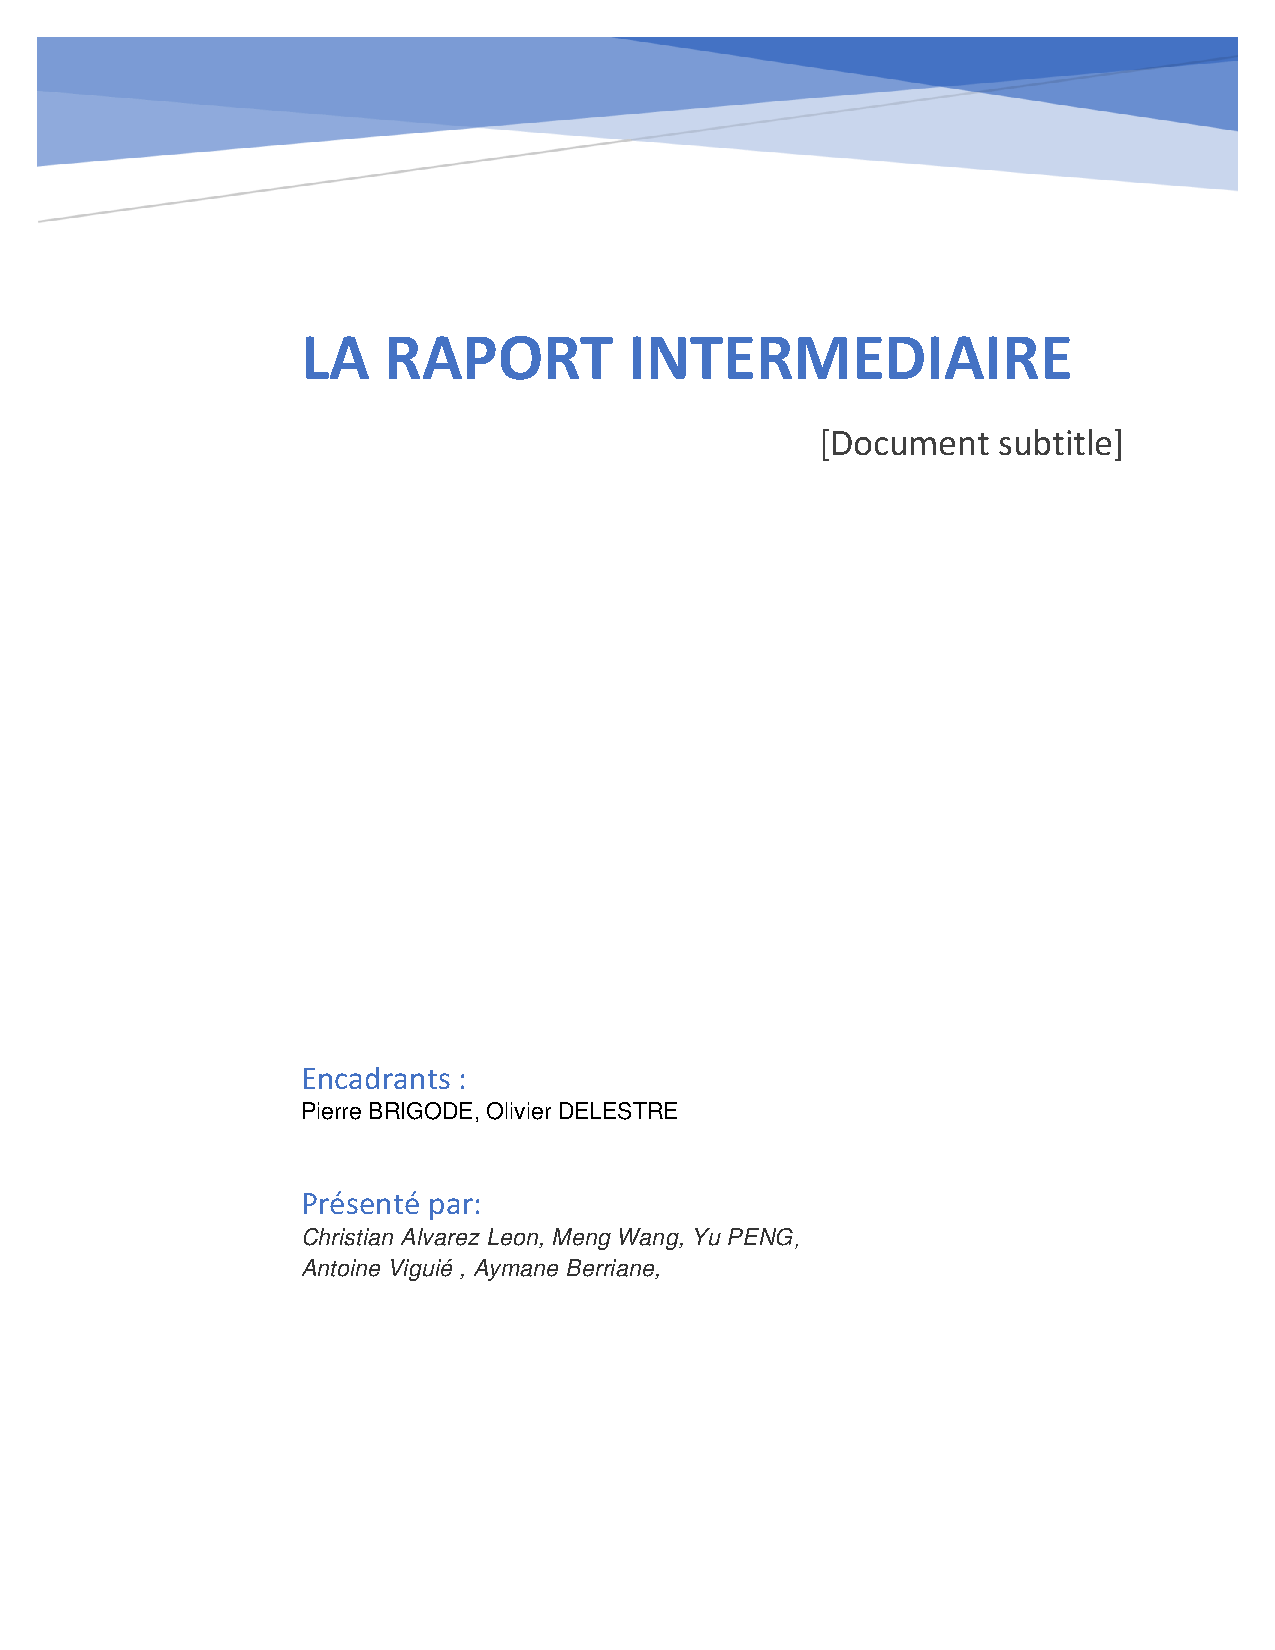
\includepdf{images/COVERPAGE.pdf}
%=======================================================================

%插入标题=================================================================
%%%\maketitle
%%=======================================================================

%加空白页但又heater
%\newpage
%\mbox{}
%\newpage



{
\setcounter{tocdepth}{2}
\tableofcontents
}


\newpage

\hypertarget{introduction}{%
\section*{Introduction}\label{introduction}}
\addcontentsline{toc}{section}{Introduction}

Dans cette annexe , on va présent une méthode de python qui a une fonctionnalité similaire au Fudda-LSPIV . Une petite rappel : La technique LSPIV (Large Scale Particle Image Velocimetry) permet de mesurer les vitesses de surface d'un écoulement par analyse de séquence d'images. La méthode LSPIV complète se compose généralement de trois parties
principales:

\begin{enumerate}
\def\labelenumi{\arabic{enumi}.}
\item
  la préparation de l'image qui permet de corriger la distorsion optique , et faire l'ortho rectification.
\item
  le traitement PIV qui permet de calculer le champ de vitesse de surface.
\item
  l'analyse des donnée qui permet en déduit le débit en utilisent le profil bathymétrique d'une section en travers et la vitesse moyennée de profondeur .
\end{enumerate}

Quand on utilisent le logiciel Fudda-LSPIV , Certain d'entre nous a rencontré des bug techniques ,Dans cette contexte , on a décidé d'utiliser Python Comme alternative. on s'intéresse par python , parce que le python nous offrit des fonctionnalité qui n'est pas intégré dans le logiciel Fudda-LSPIV , par exemple pour corriger la distorsion optique, c'est pas intégré dans Le Fudda-LSPIV mais c'est un étape essentiel. Et d'ailleurs, python est plus puissant pour analyser et traiter les donnés .

On est surtout inspiré par le rapport Flood wave monitoring using LSPIV de G.H. Gerritsen qui est publié dans Github , dans son rapport , il décit un étude de LSPIV à Chuo Kikuu, Dar es Salaam, Tanzania, Notre étude se base sur cette étude. Les données sont accessible sur Github.

\newpage

\hypertarget{ip}{%
\section*{la préparation de l'image}\label{ip}}
\addcontentsline{toc}{section}{la préparation de l'image}

La préparation de l'image est nécessaire pour être en mesure de mieux distinguer les motifs en mouvement de l'imagerie et de supprimer les effets de perspective de l'image. La manipulation d'image pour préparer l'imagerie pour l'analyse LSPIV se composent de plusieurs étapes. Subséquemment, ces étapes sont:

\begin{enumerate}
\def\labelenumi{(\arabic{enumi})}
\item
  La correction de distorsion optique.
\item
  l'orthorectification.
\item
  La mise en niveau de gris et la correction du gamma et du contraste.
\end{enumerate}

Les deux premières étapes
sont appliquées pour garantir la présence de distances égales dans les images.
La troisième étape est utilisée pour améliorer la distinction de la graine de
l'arrière-plan et donc s'assurer de la validation de similitude
processus est efficace.

Dans cette partie, on va utiliser la libraire de python Opencv3\citep{noauthor_opencv_2015} qui nous permette d'appliquer des options de manipulation d'images et le vidéo. vous pouvez l'installer par cette ligne de commande.

\begin{Shaded}
\begin{Highlighting}[]
\NormalTok{pip install opencv}\OperatorTok{{-}}\NormalTok{python}
\end{Highlighting}
\end{Shaded}

On a aussi besoin d'autres libraires python numpy, pandas, math pour traiter des données . Et si vous voulez refaire cette étude sur vos ordinateurs, On vous conseille d'utiliser le python installé de site Anaconda et jupyter notebook

\hypertarget{la-correction-de-distorsion-optique}{%
\subsection*{La correction de distorsion optique}\label{la-correction-de-distorsion-optique}}
\addcontentsline{toc}{subsection}{La correction de distorsion optique}

En raison de la la courbure des lentilles de l'appareil photo, les images peuvent être déformées. Figure \ref{fig:flens} présente les deux types de distorsions des lentilles les plus fréquentes,la distorsion en barillet et la distorsion en coussinet \citep{fryer_lens_1986} , Ces distorsions géométriques sont liées à des facteurs radiaux. Un troisième type de distorsion est distorsion tangentielle, qui se produit lorsque les lentilles ne sont pas parallèles au plan
image. Certaines caméras sont capables de faire face à ces distorsions
intérieurement. Cependant, la plupart du temps, une certaine quantité de post-traitement est
nécessaire pour ajuster les images.



\begin{figure}[H]
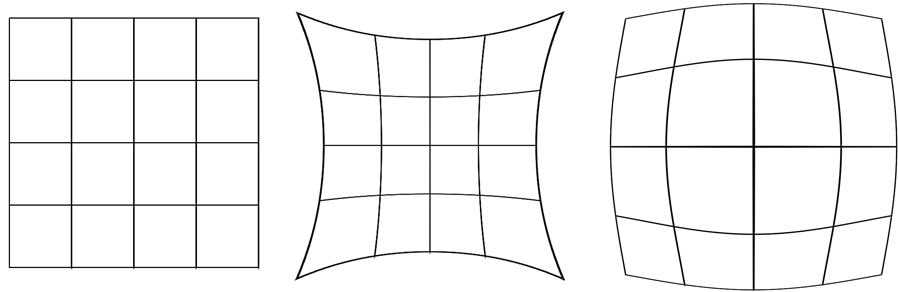
\includegraphics[width=1\linewidth,]{images/lens} \caption{Les differentes types de distortion. Du gauche à la droit : la grille d'origine, la distorsion en barillet et la distorsion en coussinet.}\label{fig:flens}
\end{figure}

Les formules suivantes sont appliquées pour supprimer la distortion radial (Voir Équation\eqref{eq:corr1}) et la distorsion tangentielle (Voir Équation\eqref{eq:corr2})

\begin{equation}
\begin{aligned}
  x_{corr} = x\left(1+k_1r^2+k_2r^4+k_3r^6\right)
  \\y_{corr} = y\left(1+k_1r^2+k_2r^4+k_3r^6\right)
\end{aligned}
 \label{eq:corr1}
\end{equation}

D'où \(𝑥\) et \(𝑦\) sont les coordonnées d'origine; \(x_{𝑐𝑜𝑟𝑟}\) et
\(y_{𝑐𝑜𝑟𝑟}\) sont les coordonnées corrigés. \(𝑟\) est la distance entre le
point \(\left(𝑥, 𝑦\right)\) et le centre de la distortion. \(𝑘_1\), \(𝑘_2\),
et \(𝑘_3\) sont les coefficients radiales. Pour la distortion en barillet et la distortion en coussinet , \(𝑘_1\) est respectivemen negative et positive. \(𝑘_2\) et \(𝑘_3\) sont négligeables.

\begin{equation}
\begin{aligned}
   x_{corr} = x+\left[ 2 p_1 x y+ p_2\left( r^2+2x^2\right) \right]\\
  y_{corr} = y+\left[ p_1 \left(r^2+2 y^2\right)+ 2p_2xy\right]
\end{aligned}
 \label{eq:corr2}
\end{equation}

D'où \(𝑝_1\) et \(𝑝_2\) sont les coefficient de la distortion tangentielle. les différents coefficients sont souvent stockés dans un tableau:

\begin{equation}
C_{dis}=
\begin{bmatrix}
k_1 & k_2 & p_1 & p_2 & k_3
\end{bmatrix}
\end{equation}

À part du coefficient de distorsion, pour pouvoir corriger l'imagerie, Une conversion entre les coordonnées de distorsion et la résolution de la caméra est
fait. Pour cela, la formule est donnée dans l'équation \eqref{eq:corr3}

\begin{equation}
\begin{bmatrix}
x\\
y\\
w
\end{bmatrix}
= M_{con} \cdot
\begin{bmatrix}
x\\
y\\
z
\end{bmatrix}
\quad \text{d'où} \quad
M_{con} =
\begin{bmatrix}
f_x & 0 & c_x\\
0 & f_y & c_y\\
0 & 0 &1
\end{bmatrix}
\label{eq:corr3}
\end{equation}

D'où \([𝑥, 𝑦, 𝑤]\) sont les coordonnées d'image homogène 2D et \([x, y , z]\) sont les coordonnées de caméra 3D . \(f_𝑥\) et \(𝑓_𝑦\) sont les longueurs locales de la caméra dans le sens \(𝑥\) et \(𝑦\) ,en genéral, ils sont identiques \(𝑐_𝑥\) et \(𝑐_𝑦\) sont les coordinations de centre optique de la caméra dans le sens \(𝑥\) et \(𝑦\).

\begin{Shaded}
\begin{Highlighting}[]
\OperatorTok{\%}\NormalTok{matplotlib inline}
\end{Highlighting}
\end{Shaded}

\begin{Shaded}
\begin{Highlighting}[]
\ImportTok{import}\NormalTok{ numpy }\ImportTok{as}\NormalTok{ np}
\ImportTok{import}\NormalTok{ os}
\ImportTok{import}\NormalTok{ matplotlib.pyplot }\ImportTok{as}\NormalTok{ plt}
\ImportTok{import}\NormalTok{ pandas }\ImportTok{as}\NormalTok{ pd}
\ImportTok{import}\NormalTok{ cv2}
\end{Highlighting}
\end{Shaded}

\begin{Shaded}
\begin{Highlighting}[]
\NormalTok{dir\_video }\OperatorTok{=} \StringTok{\textquotesingle{}Python/example\_video.mp4\textquotesingle{}}
\NormalTok{dir\_saves }\OperatorTok{=} \StringTok{\textquotesingle{}Python/frames\textquotesingle{}}
\end{Highlighting}
\end{Shaded}

\begin{Shaded}
\begin{Highlighting}[]
\ControlFlowTok{if} \KeywordTok{not}\NormalTok{ os.path.exists(dir\_saves):}
\NormalTok{    os.mkdir(dir\_saves)}
\end{Highlighting}
\end{Shaded}

\begin{Shaded}
\begin{Highlighting}[]
\CommentTok{\# définition de correction de la distorsion }
\KeywordTok{def}\NormalTok{ lens\_corr(img, k1}\OperatorTok{={-}}\FloatTok{10.0e{-}6}\NormalTok{, c}\OperatorTok{=}\DecValTok{2}\NormalTok{, f}\OperatorTok{=}\FloatTok{8.0}\NormalTok{):}
 
    \CommentTok{\# définition la caractère de l\textquotesingle{}image }
\NormalTok{    height, width, \_\_ }\OperatorTok{=}\NormalTok{ img.shape}

    \CommentTok{\# le vecteur de coefficient de distorsion}
\NormalTok{    dist }\OperatorTok{=}\NormalTok{ np.zeros((}\DecValTok{5}\NormalTok{,}\DecValTok{1}\NormalTok{),np.float64)}
\NormalTok{    dist[}\DecValTok{0}\NormalTok{,}\DecValTok{0}\NormalTok{] }\OperatorTok{=}\NormalTok{ k1}
    
    \CommentTok{\# la matrice du caméra}
\NormalTok{    mtx }\OperatorTok{=}\NormalTok{ np.eye(}\DecValTok{3}\NormalTok{,dtype}\OperatorTok{=}\NormalTok{np.float32)}

\NormalTok{    mtx[}\DecValTok{0}\NormalTok{,}\DecValTok{2}\NormalTok{] }\OperatorTok{=}\NormalTok{ width}\OperatorTok{/}\NormalTok{c     }\CommentTok{\# centre x}
\NormalTok{    mtx[}\DecValTok{1}\NormalTok{,}\DecValTok{2}\NormalTok{] }\OperatorTok{=}\NormalTok{ height}\OperatorTok{/}\NormalTok{c    }\CommentTok{\# centre y}
\NormalTok{    mtx[}\DecValTok{0}\NormalTok{,}\DecValTok{0}\NormalTok{] }\OperatorTok{=}\NormalTok{ f           }\CommentTok{\# la distance focale x}
\NormalTok{    mtx[}\DecValTok{1}\NormalTok{,}\DecValTok{1}\NormalTok{] }\OperatorTok{=}\NormalTok{ f           }\CommentTok{\# la distance focale y}

    \CommentTok{\# la correction d\textquotesingle{}image par la distorsion}
\NormalTok{    corr\_img }\OperatorTok{=}\NormalTok{ cv2.undistort(img, mtx, dist)}

    \ControlFlowTok{return}\NormalTok{ corr\_img}
\end{Highlighting}
\end{Shaded}

\begin{Shaded}
\begin{Highlighting}[]
\CommentTok{\# pour localiser les GCPts dans les images:}
\CommentTok{\# importer la vidéo et corriger la première image pour la distorsion de l\textquotesingle{}objectif}
\NormalTok{cap }\OperatorTok{=}\NormalTok{ cv2.VideoCapture(dir\_video)}
\ControlFlowTok{if}\NormalTok{ cap.isOpened():}
\NormalTok{    ret, img }\OperatorTok{=}\NormalTok{ cap.read()}
\NormalTok{    corr\_img }\OperatorTok{=}\NormalTok{ lens\_corr(img, k1}\OperatorTok{={-}}\FloatTok{10.0e{-}6}\NormalTok{, c}\OperatorTok{=}\DecValTok{2}\NormalTok{, f}\OperatorTok{=}\FloatTok{8.0}\NormalTok{)}
\NormalTok{cap.release()}

\CommentTok{\# afficher l\textquotesingle{}image corrigée et les emplacements des GCP}
\NormalTok{fig }\OperatorTok{=}\NormalTok{ plt.figure(figsize}\OperatorTok{=}\NormalTok{(}\DecValTok{14}\NormalTok{,}\DecValTok{5}\NormalTok{))}
\NormalTok{plt.subplots\_adjust(left}\OperatorTok{=}\DecValTok{0}\NormalTok{, bottom}\OperatorTok{=}\DecValTok{0}\NormalTok{, right}\OperatorTok{=}\DecValTok{1}\NormalTok{, top}\OperatorTok{=}\DecValTok{1}\NormalTok{, wspace}\OperatorTok{=}\FloatTok{0.1}\NormalTok{, hspace}\OperatorTok{=}\DecValTok{0}\NormalTok{)}
\CommentTok{\# [:,:,::{-}1] BGR =\textgreater{} RGB ; Dans opencv c\textquotesingle{}est BGR}
\NormalTok{plt.subplot(}\DecValTok{121}\NormalTok{)}
\NormalTok{plt.imshow(img[:,:,::}\OperatorTok{{-}}\DecValTok{1}\NormalTok{])}
\NormalTok{plt.title(}\StringTok{\textquotesingle{}AVANT\textquotesingle{}}\NormalTok{)}
\NormalTok{plt.axis(}\StringTok{\textquotesingle{}off\textquotesingle{}}\NormalTok{) }
\end{Highlighting}
\end{Shaded}

\begin{verbatim}
## (-0.5, 1919.5, 1079.5, -0.5)
\end{verbatim}

\begin{Shaded}
\begin{Highlighting}[]
\NormalTok{plt.subplot(}\DecValTok{122}\NormalTok{)}
\NormalTok{plt.imshow(corr\_img[:,:,::}\OperatorTok{{-}}\DecValTok{1}\NormalTok{])}
\NormalTok{plt.title(}\StringTok{\textquotesingle{}APRÈS\textquotesingle{}}\NormalTok{)}
\NormalTok{plt.axis(}\StringTok{\textquotesingle{}off\textquotesingle{}}\NormalTok{) }
\end{Highlighting}
\end{Shaded}

\begin{verbatim}
## (-0.5, 1919.5, 1079.5, -0.5)
\end{verbatim}

\begin{Shaded}
\begin{Highlighting}[]
\NormalTok{plt.show()}
\end{Highlighting}
\end{Shaded}

\begin{figure}[H]
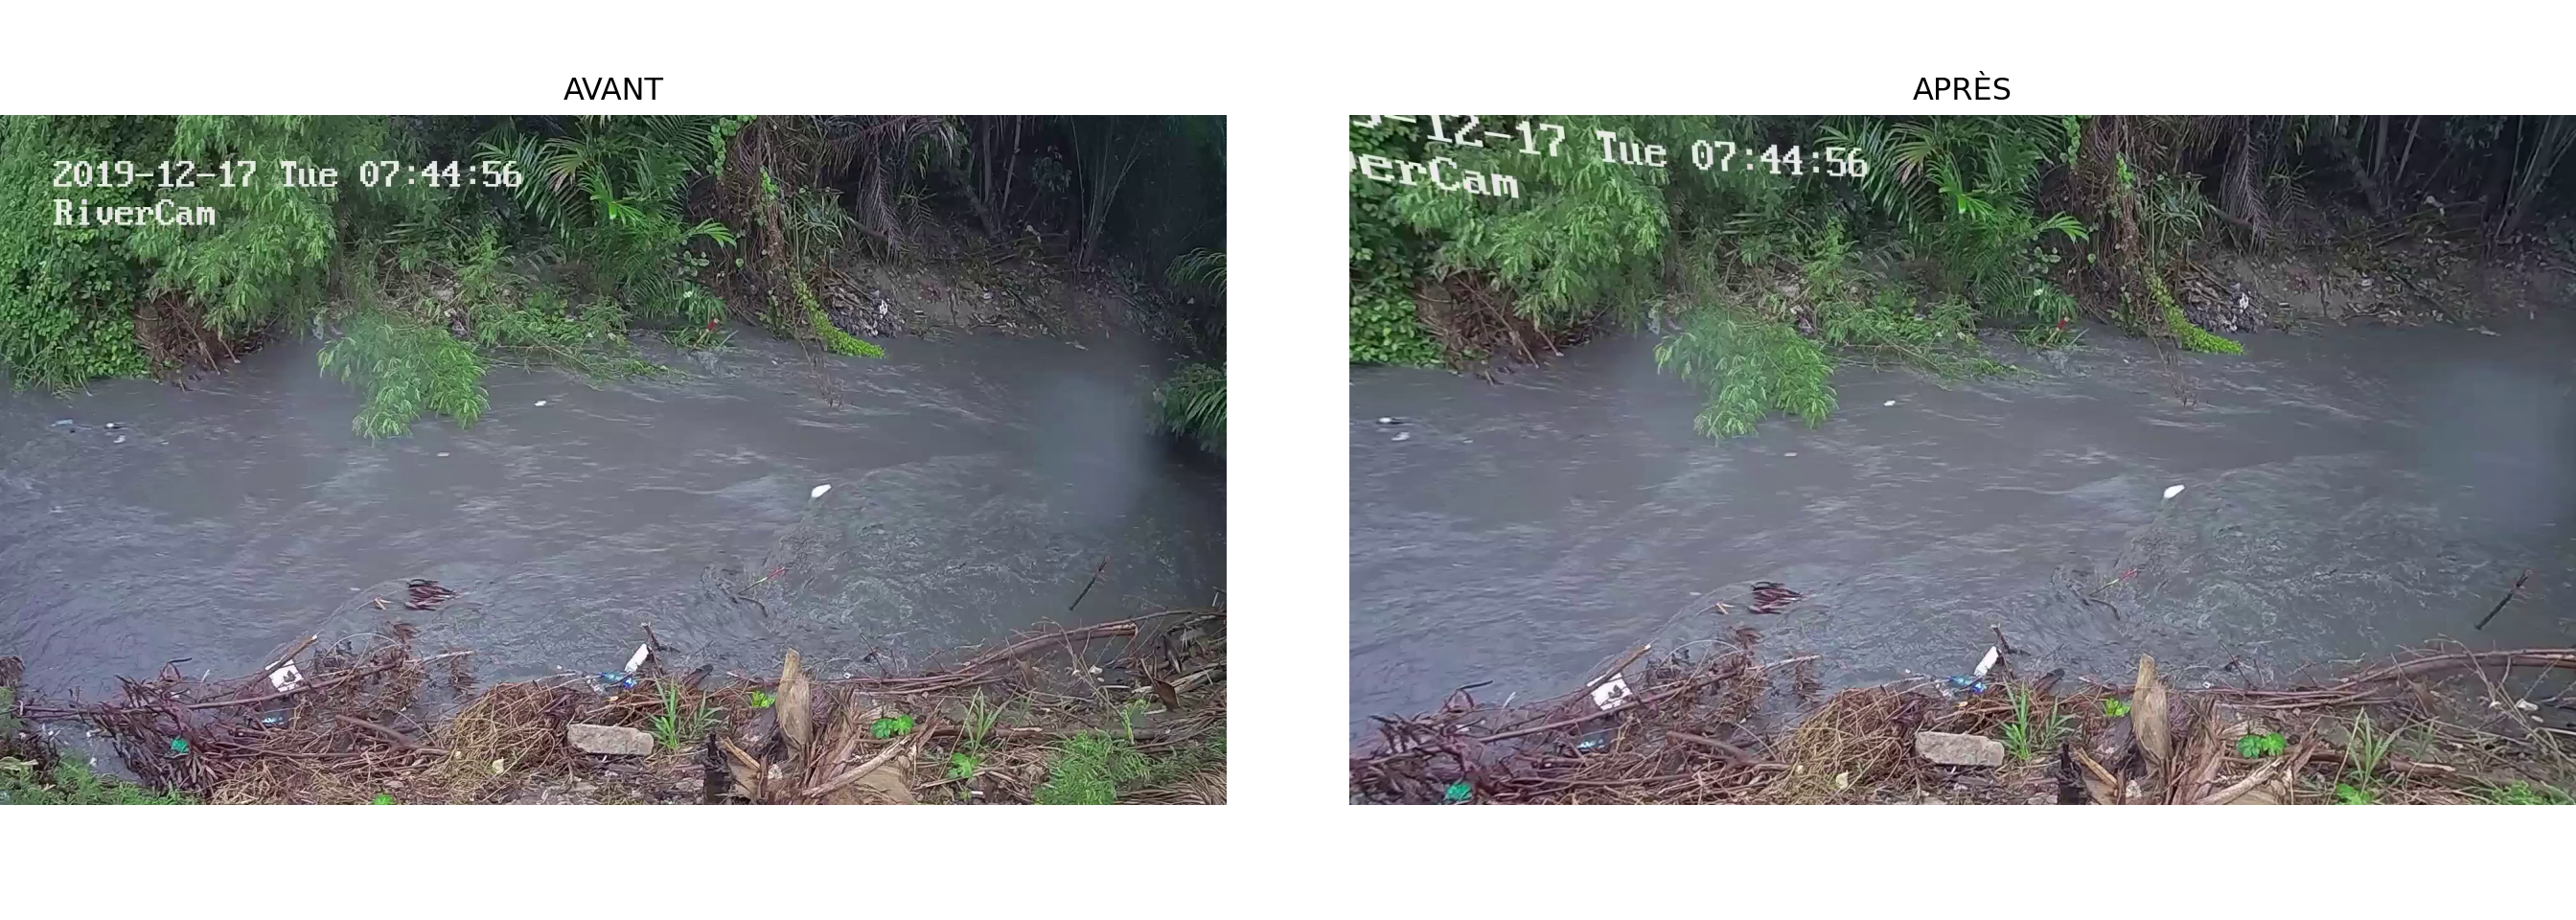
\includegraphics[width=1\linewidth,]{PROJET_LSPIV_files/figure-latex/unnamed-chunk-8-1} \caption{La correction de distorsion optique}\label{fig:unnamed-chunk-8}
\end{figure}

\hypertarget{lorthorectification}{%
\subsection*{l'orthorectification}\label{lorthorectification}}
\addcontentsline{toc}{subsection}{l'orthorectification}

Pour supprimer les effets de la perspective de l'image ,( où les objets sont plus proches
de la caméra semble être plus grande dans l'image) ,l'orthorectification est appliquée.
Lors de l'application d'orthorectification,le système de coordonnées de l'imagerie est transféré à une système de coordonnée locale. Pour ce système de coordonnées locales, points de contrôle au sol (GCP) sont
mis en place à côté du flux sont utilisés. Pour l'orthorectification
processus pour être aussi précis que possible, au moins quatre GCP sont nécessaires, si
les images sont capturées perpendiculairement au flux ou lorsque les GCP
sont placés au même niveau que le niveau de l'eau. Un minimum de six
GCP sont nécessaires lorsque les GCP ne sont pas placés dans le même plan que le
niveau d'eau. Sur la Figure \ref{fig:fortho} les différents sites de jaugeage
et les configurations sont affichées.



\begin{figure}[H]
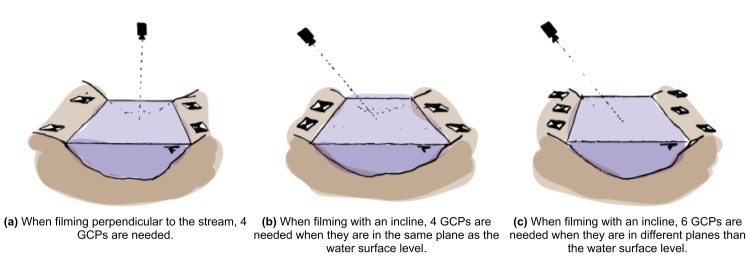
\includegraphics[width=1\linewidth,]{images/ortho} \caption{Nombre de points de contrôle au sol (GCP) nécessaires dans différentes circonstances.(source: Flood wave monitoring using LSPIV)}\label{fig:fortho}
\end{figure}

Lors de l'utilisation de quatre GCP, les facteurs d'inversion \(𝑓_𝑥\) et \(𝑓_𝑦\) sont
déterminé en utilisant la formule indiquée dans l'équation \eqref{eq:corr4}.

\begin{equation}
p_{loc}\left(x,y\right)=p_{img}\left(f_x\left(x,y\right), f_y\left(x,y\right)\right)
\label{eq:corr4}
\end{equation}

D'où \(𝑝_ {𝑑𝑠𝑡} \left (𝑥, 𝑦, 𝑧 \right)\) est l'emplacement géographique du
point de contrôle au sol dans le système de coordonnées local, généralement en métrique
units; \(𝑝_ {𝑠𝑟𝑐} \left (𝑥, 𝑦 \right)\) est la coordonnée xy du sol
point de contrôle dans l'imagerie, généralement en pixels; et \(𝑓_𝑥\) et \(𝑓_𝑦\) le
facteurs d'inversion.

Simultanément à ce processus, la résolution de l'image peut être réglée
en multipliant les coordonnées \(𝐺𝐶𝑃_ {𝑑𝑠𝑡} \left (𝑥, 𝑦 \right)\) par les
pixels souhaités par coefficient de mètre.

Lorsque six (ou plus) GCP sont utilisés - parce que les coordonnées en trois dimensions
pour les GCP sont nécessaires - un modèle de sténopé peut être utilisé. Cette méthode est
expliqué par \citep{jodeau_application_2008}

\begin{Shaded}
\begin{Highlighting}[]
\CommentTok{\# Emplacements des GCPs dans les images (pixels)}
\NormalTok{data\_from }\OperatorTok{=}\NormalTok{ \{}\StringTok{\textquotesingle{}x\textquotesingle{}}\NormalTok{: [}\DecValTok{992}\NormalTok{, }\DecValTok{1545}\NormalTok{, }\DecValTok{1773}\NormalTok{,  }\DecValTok{943}\NormalTok{],}
             \StringTok{\textquotesingle{}y\textquotesingle{}}\NormalTok{: [}\DecValTok{366}\NormalTok{,  }\DecValTok{403}\NormalTok{,  }\DecValTok{773}\NormalTok{,  }\DecValTok{724}\NormalTok{]\}}
\NormalTok{df\_from }\OperatorTok{=}\NormalTok{ pd.DataFrame(data\_from)}


\NormalTok{fig }\OperatorTok{=}\NormalTok{ plt.figure(figsize}\OperatorTok{=}\NormalTok{(}\DecValTok{7}\NormalTok{,}\DecValTok{4}\NormalTok{))}
\NormalTok{plt.subplot(}\DecValTok{111}\NormalTok{)}
\NormalTok{plt.subplots\_adjust(left}\OperatorTok{=}\DecValTok{0}\NormalTok{, bottom}\OperatorTok{=}\DecValTok{0}\NormalTok{, right}\OperatorTok{=}\DecValTok{1}\NormalTok{, top}\OperatorTok{=}\DecValTok{1}\NormalTok{, wspace}\OperatorTok{=}\FloatTok{0.1}\NormalTok{, hspace}\OperatorTok{=}\DecValTok{0}\NormalTok{)}
\NormalTok{plt.imshow(corr\_img[:,:,::}\OperatorTok{{-}}\DecValTok{1}\NormalTok{])}
\NormalTok{plt.plot(df\_from.x, df\_from.y ,}\StringTok{\textquotesingle{}r.\textquotesingle{}}\NormalTok{)}
\NormalTok{plt.axis(}\StringTok{\textquotesingle{}off\textquotesingle{}}\NormalTok{)}
\end{Highlighting}
\end{Shaded}

\begin{verbatim}
## (-0.5, 1919.5, 1079.5, -0.5)
\end{verbatim}

\begin{Shaded}
\begin{Highlighting}[]
\NormalTok{plt.show()}
\end{Highlighting}
\end{Shaded}

\begin{figure}[H]
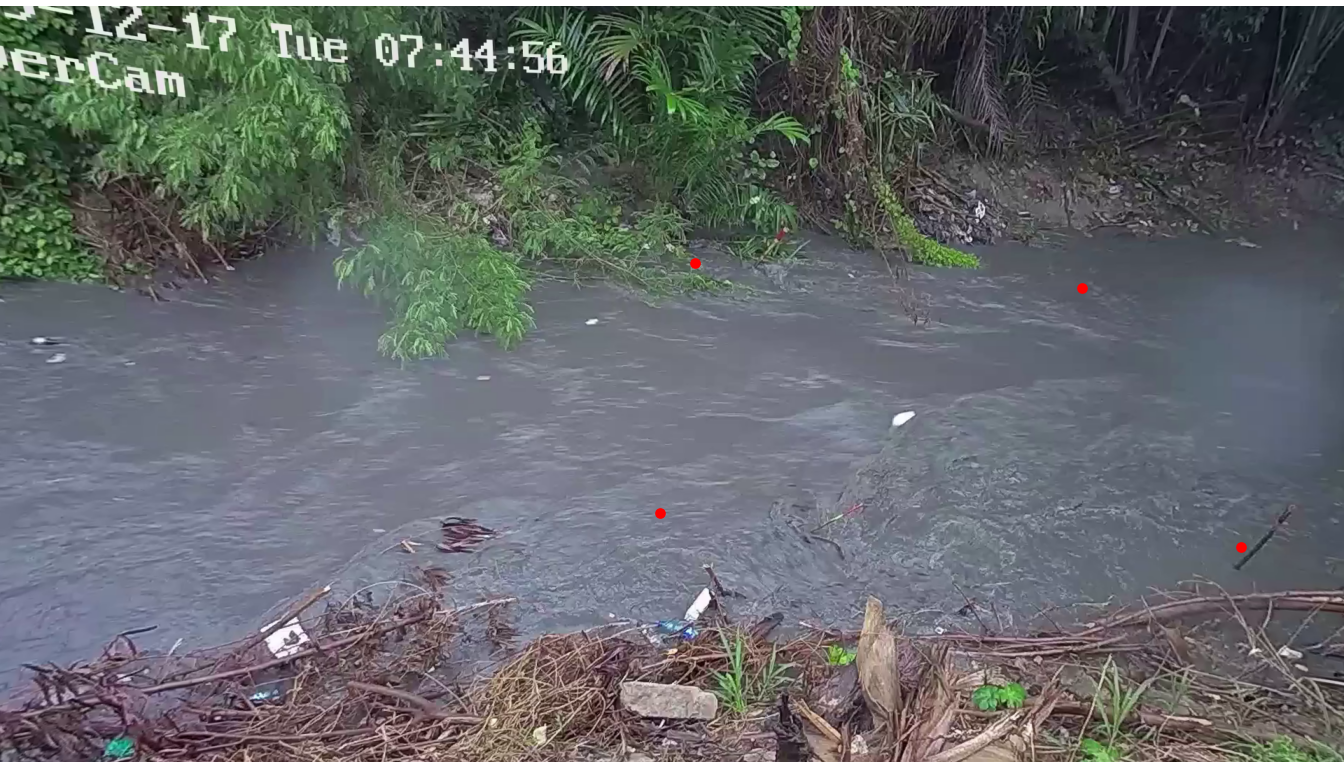
\includegraphics[width=1\linewidth,]{PROJET_LSPIV_files/figure-latex/unnamed-chunk-9-1} \caption{Les localisations des GRPS}\label{fig:unnamed-chunk-9}
\end{figure}

\begin{Shaded}
\begin{Highlighting}[]
\CommentTok{\# Emplacements des GCPs dans le système de coordonnées local (mètres)}
\NormalTok{data\_to }\OperatorTok{=}\NormalTok{ \{}\StringTok{\textquotesingle{}x\textquotesingle{}}\NormalTok{: [ }\FloatTok{0.25}\NormalTok{, }\FloatTok{4.25}\NormalTok{, }\FloatTok{4.50}\NormalTok{, }\FloatTok{0.00}\NormalTok{],}
           \StringTok{\textquotesingle{}y\textquotesingle{}}\NormalTok{: [ }\FloatTok{0.30}\NormalTok{, }\FloatTok{0.20}\NormalTok{, }\FloatTok{3.50}\NormalTok{, }\FloatTok{3.50}\NormalTok{]\}}
\NormalTok{df\_to }\OperatorTok{=}\NormalTok{ pd.DataFrame(data\_to)}
\end{Highlighting}
\end{Shaded}

\begin{Shaded}
\begin{Highlighting}[]
\KeywordTok{def}\NormalTok{ orthorect\_param(img, df\_from, df\_to, PPM}\OperatorTok{=}\DecValTok{100}\NormalTok{):}
    
    \CommentTok{\# définir le valeur de float32(par point)}
\NormalTok{    pts1 }\OperatorTok{=}\NormalTok{ np.float32(df\_from.values)}
\NormalTok{    pts2 }\OperatorTok{=}\NormalTok{ np.float32(df\_to.values }\OperatorTok{*}\NormalTok{ PPM)}

    \CommentTok{\# définir une matrice de transformation basée sur les GCP}
\NormalTok{    M }\OperatorTok{=}\NormalTok{ cv2.getPerspectiveTransform(pts1, pts2)}

    \CommentTok{\# trouver les emplacements des coins d\textquotesingle{}image transformés}
\NormalTok{    height, width, \_\_ }\OperatorTok{=}\NormalTok{ img.shape}
\NormalTok{    C }\OperatorTok{=}\NormalTok{ np.array([[}\DecValTok{0}\NormalTok{, }\DecValTok{0}\NormalTok{, }\DecValTok{1}\NormalTok{],}
\NormalTok{                  [width, }\DecValTok{0}\NormalTok{, }\DecValTok{1}\NormalTok{],}
\NormalTok{                  [}\DecValTok{0}\NormalTok{, height, }\DecValTok{1}\NormalTok{],}
\NormalTok{                  [width, height, }\DecValTok{1}\NormalTok{]])}
\NormalTok{    C\_new }\OperatorTok{=}\NormalTok{ np.array([(np.dot(i, M.T) }\OperatorTok{/}\NormalTok{ np.dot(i, M.T)[}\DecValTok{2}\NormalTok{])[:}\DecValTok{2}\NormalTok{] }\ControlFlowTok{for}\NormalTok{ i }\KeywordTok{in}\NormalTok{ C])}

\NormalTok{    C\_new[:, }\DecValTok{0}\NormalTok{] }\OperatorTok{{-}=} \BuiltInTok{min}\NormalTok{(C\_new[:, }\DecValTok{0}\NormalTok{])}
\NormalTok{    C\_new[:, }\DecValTok{1}\NormalTok{] }\OperatorTok{{-}=} \BuiltInTok{min}\NormalTok{(C\_new[:, }\DecValTok{1}\NormalTok{])}
    
    \CommentTok{\# définir une nouvelle matrice de transformation basée sur les coins de l\textquotesingle{}image}
    \CommentTok{\# sinon, une partie des images ne sera pas enregistrée}
\NormalTok{    M\_new }\OperatorTok{=}\NormalTok{ cv2.getPerspectiveTransform(np.float32(C[:,:}\DecValTok{2}\NormalTok{]), np.float32(C\_new))}

    \ControlFlowTok{return}\NormalTok{ M\_new, C\_new, df\_to}
\end{Highlighting}
\end{Shaded}

\begin{Shaded}
\begin{Highlighting}[]
\CommentTok{\#déterminer les paramètres d\textquotesingle{}orthorectification}
\NormalTok{M, C, \_\_ }\OperatorTok{=}\NormalTok{ orthorect\_param(corr\_img, df\_from, df\_to, PPM}\OperatorTok{=}\DecValTok{100}\NormalTok{)}

\CommentTok{\# définir la taille de l\textquotesingle{}image orthorectifiée}
\NormalTok{cols }\OperatorTok{=} \BuiltInTok{int}\NormalTok{(np.ceil(}\BuiltInTok{max}\NormalTok{(C[:, }\DecValTok{0}\NormalTok{])))}
\NormalTok{rows }\OperatorTok{=} \BuiltInTok{int}\NormalTok{(np.ceil(}\BuiltInTok{max}\NormalTok{(C[:, }\DecValTok{1}\NormalTok{])))}


\CommentTok{\# orthorectifier l\textquotesingle{}image}

\NormalTok{fig }\OperatorTok{=}\NormalTok{ plt.figure(figsize}\OperatorTok{=}\NormalTok{(}\DecValTok{7}\NormalTok{,}\DecValTok{4}\NormalTok{))}
\NormalTok{plt.subplots\_adjust(left}\OperatorTok{=}\DecValTok{0}\NormalTok{, bottom}\OperatorTok{=}\DecValTok{0}\NormalTok{, right}\OperatorTok{=}\DecValTok{1}\NormalTok{, top}\OperatorTok{=}\DecValTok{1}\NormalTok{, wspace}\OperatorTok{=}\FloatTok{0.1}\NormalTok{, hspace}\OperatorTok{=}\DecValTok{0}\NormalTok{)}

\NormalTok{plt.subplot(}\DecValTok{111}\NormalTok{)}
\NormalTok{ortho\_img }\OperatorTok{=}\NormalTok{ cv2.warpPerspective(img, M, (cols, rows))}
\NormalTok{plt.imshow(ortho\_img[:,:,::}\OperatorTok{{-}}\DecValTok{1}\NormalTok{])}
\NormalTok{plt.axis(}\StringTok{\textquotesingle{}off\textquotesingle{}}\NormalTok{)}
\end{Highlighting}
\end{Shaded}

\begin{verbatim}
## (-0.5, 2085.5, 1516.5, -0.5)
\end{verbatim}

\begin{Shaded}
\begin{Highlighting}[]
\NormalTok{plt.show()}
\end{Highlighting}
\end{Shaded}

\begin{figure}[H]
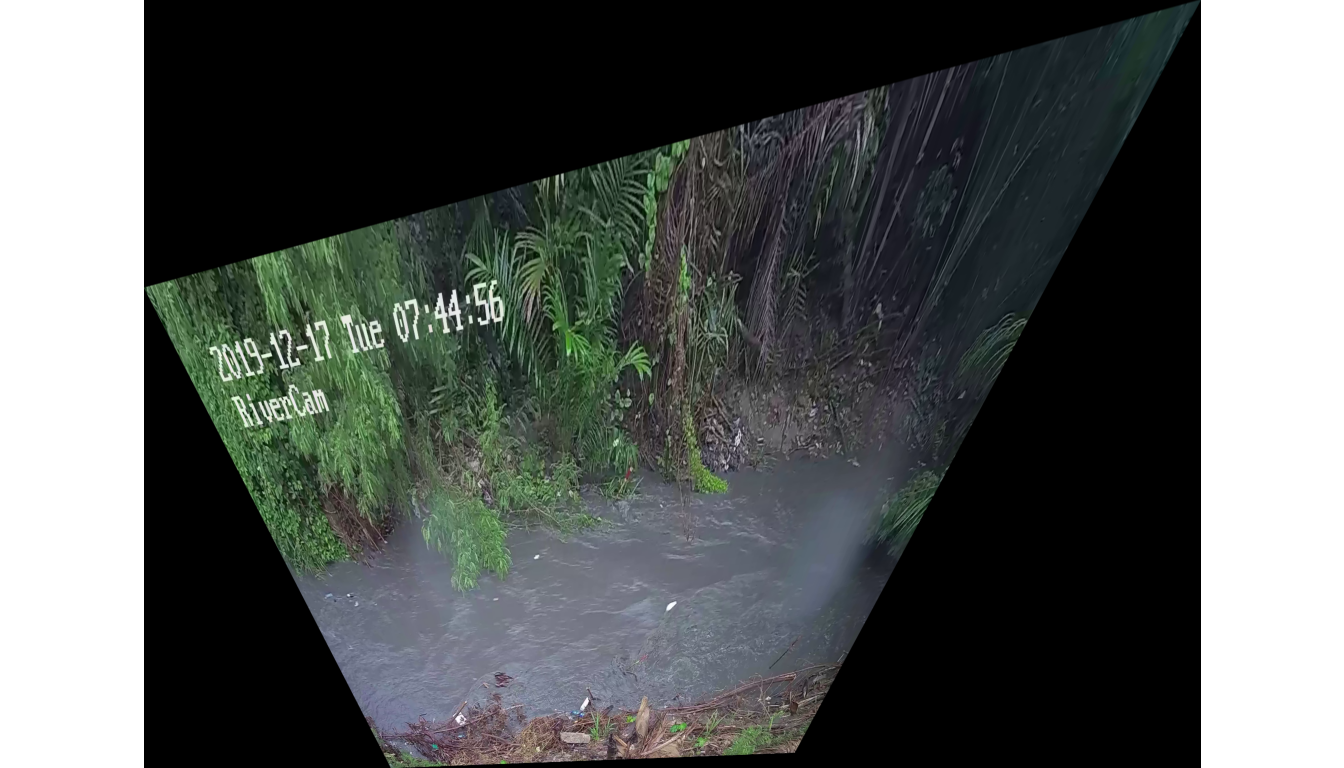
\includegraphics[width=1\linewidth,]{PROJET_LSPIV_files/figure-latex/unnamed-chunk-12-1} \caption{L'orthorectification}\label{fig:unnamed-chunk-12}
\end{figure}

\hypertarget{la-mise-en-niveau-de-gris-et-la-correction-du-gamma-et-du-contraste.}{%
\subsection*{La mise en niveau de gris et la correction du gamma et du contraste.}\label{la-mise-en-niveau-de-gris-et-la-correction-du-gamma-et-du-contraste.}}
\addcontentsline{toc}{subsection}{La mise en niveau de gris et la correction du gamma et du contraste.}

La dernière étape de la préparation de l'image est la conversion du
imagerie à une échelle de gris et pour appliquer une correction de contraste et gamma.
Une mise à l'échelle des gris est nécessaire pour pouvoir appliquer la validation de similarité entre
images vidéo séquentielles. La correction de contraste et gamma est appliquée à
améliorer la visibilité des semences. Les corrections de contraste et gamma sont
appliqué à l'aide des formules suivantes:

\begin{equation}
O_{constract} = \alpha \cdot I + \beta
\label{eq:constract}
\end{equation}

\begin{equation}
O_{gamma} = \left(\frac{I}{255}\right)^\frac{1}{\gamma} \cdot 255
\label{eq:gamma}
\end{equation}

D'où \(\alpha\) et \(\beta\) définit la correction du contraste; \(\gamma\) est la correction de gamma; \(O_n\) sont les imageries corrigés; et \(I\) est l'imagerie d'origine.

\begin{Shaded}
\begin{Highlighting}[]
\NormalTok{gamma}\OperatorTok{=}\FloatTok{0.4}

\CommentTok{\# transformer l\textquotesingle{}image en niveaux de gris}
\NormalTok{Grey\_img }\OperatorTok{=}\NormalTok{ cv2.cvtColor(ortho\_img, cv2.COLOR\_BGR2GRAY)}

\CommentTok{\# appliquer la correction gamma}
\NormalTok{invGamma }\OperatorTok{=} \FloatTok{1.}\OperatorTok{/}\NormalTok{gamma}
\NormalTok{table }\OperatorTok{=}\NormalTok{ (np.array([((i }\OperatorTok{/} \FloatTok{255.0}\NormalTok{) }\OperatorTok{**}\NormalTok{ invGamma) }\OperatorTok{*} \DecValTok{255} 
            \ControlFlowTok{for}\NormalTok{ i }\KeywordTok{in}\NormalTok{ np.arange(}\DecValTok{0}\NormalTok{, }\DecValTok{256}\NormalTok{)]).astype(}\StringTok{\textquotesingle{}uint8\textquotesingle{}}\NormalTok{))}
    
\NormalTok{Gamma\_img }\OperatorTok{=}\NormalTok{ cv2.LUT(Grey\_img, table)}


\NormalTok{fig }\OperatorTok{=}\NormalTok{ plt.figure(figsize}\OperatorTok{=}\NormalTok{(}\DecValTok{14}\NormalTok{,}\DecValTok{4}\NormalTok{))}
\NormalTok{plt.subplots\_adjust(left}\OperatorTok{=}\DecValTok{0}\NormalTok{, bottom}\OperatorTok{=}\DecValTok{0}\NormalTok{, right}\OperatorTok{=}\DecValTok{1}\NormalTok{, top}\OperatorTok{=}\DecValTok{1}\NormalTok{, wspace}\OperatorTok{=}\FloatTok{0.1}\NormalTok{, hspace}\OperatorTok{=}\DecValTok{0}\NormalTok{)}

\NormalTok{plt.subplot(}\DecValTok{121}\NormalTok{)}
\NormalTok{plt.imshow(Grey\_img,cmap}\OperatorTok{=}\StringTok{"gray"}\NormalTok{)}
\NormalTok{plt.title(}\StringTok{\textquotesingle{}GRAY SCALE\textquotesingle{}}\NormalTok{)}
\NormalTok{plt.axis(}\StringTok{\textquotesingle{}off\textquotesingle{}}\NormalTok{) }
\end{Highlighting}
\end{Shaded}

\begin{verbatim}
## (-0.5, 2085.5, 1516.5, -0.5)
\end{verbatim}

\begin{Shaded}
\begin{Highlighting}[]
\NormalTok{plt.subplot(}\DecValTok{122}\NormalTok{)}
\NormalTok{plt.imshow(Gamma\_img, }\StringTok{\textquotesingle{}gray\textquotesingle{}}\NormalTok{)}
\NormalTok{plt.title(}\StringTok{\textquotesingle{}GAMMA\textquotesingle{}}\NormalTok{)}
\NormalTok{plt.axis(}\StringTok{\textquotesingle{}off\textquotesingle{}}\NormalTok{) }
\end{Highlighting}
\end{Shaded}

\begin{verbatim}
## (-0.5, 2085.5, 1516.5, -0.5)
\end{verbatim}

\begin{Shaded}
\begin{Highlighting}[]
\NormalTok{plt.show()}
\end{Highlighting}
\end{Shaded}

\begin{figure}[H]
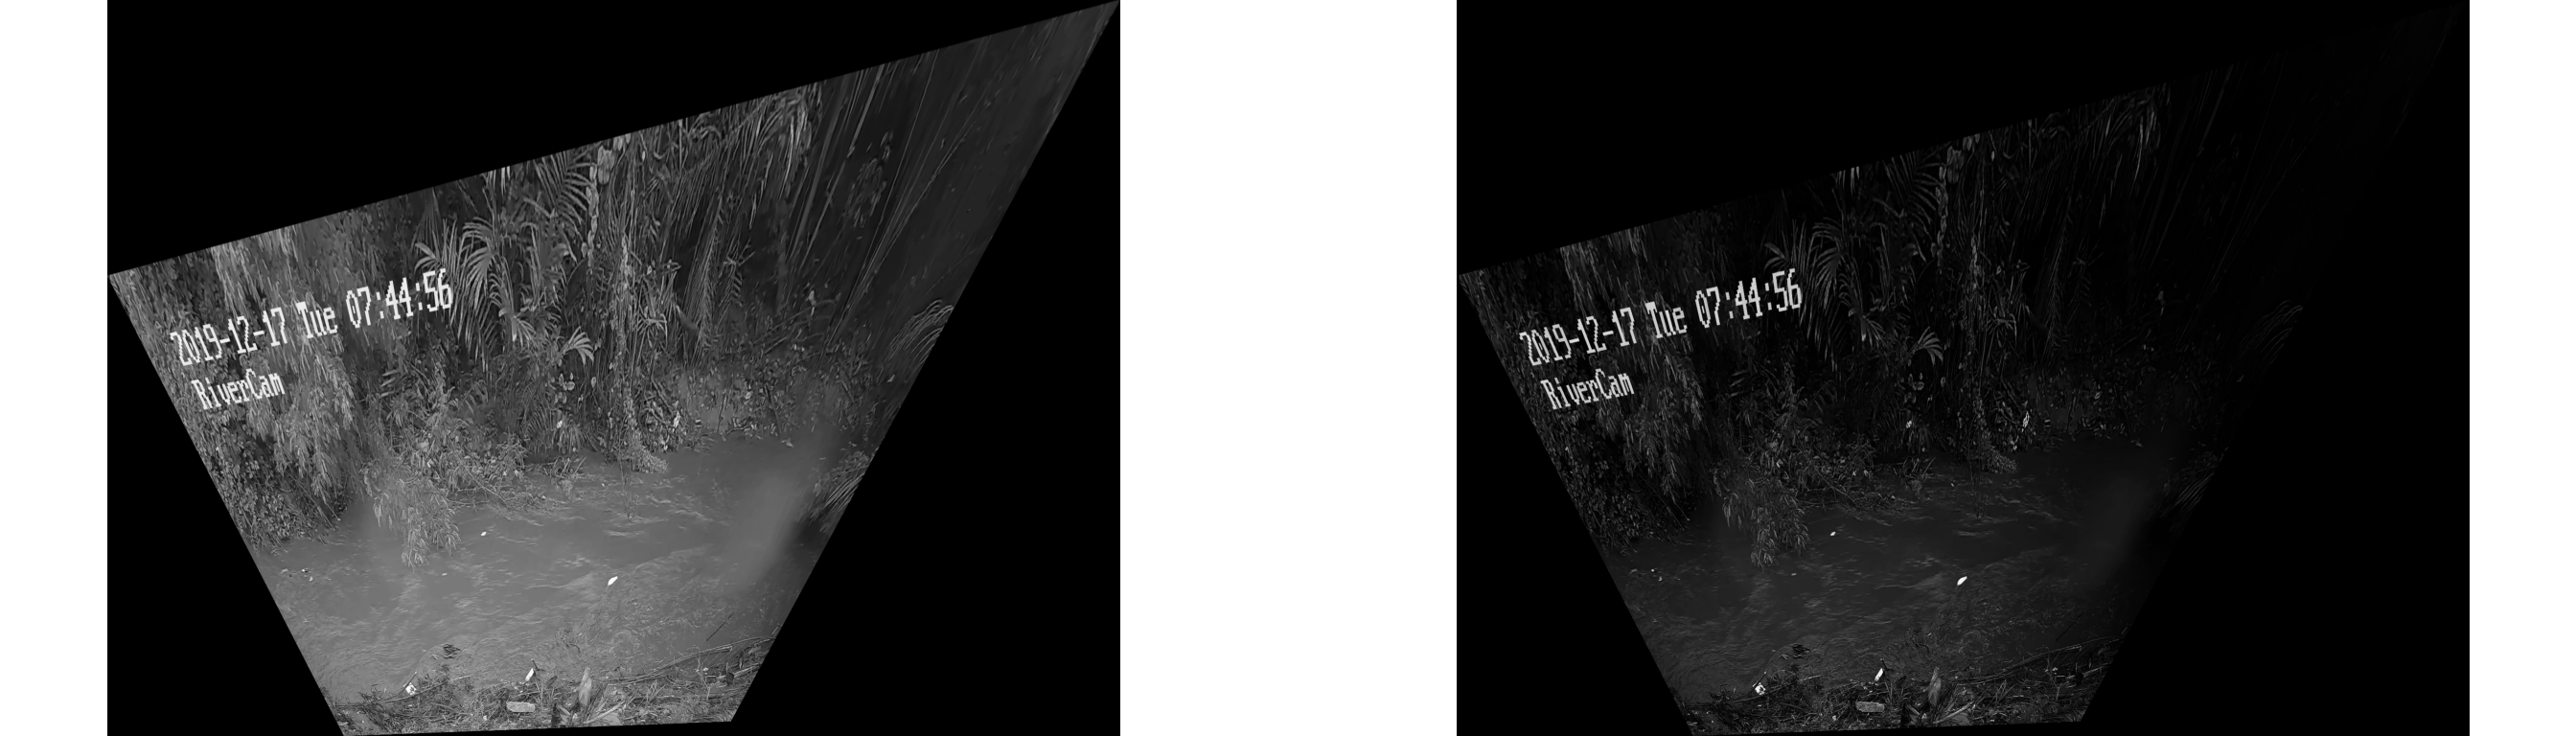
\includegraphics[width=1\linewidth,]{PROJET_LSPIV_files/figure-latex/unnamed-chunk-13-1} \caption{L'orthorectification}\label{fig:unnamed-chunk-13}
\end{figure}

\hypertarget{pour-tous-les-images}{%
\subsection*{Pour tous les images}\label{pour-tous-les-images}}
\addcontentsline{toc}{subsection}{Pour tous les images}

\begin{Shaded}
\begin{Highlighting}[]
\CommentTok{\# compteur à utiliser comme nom pour les images individuelles}
\NormalTok{n }\OperatorTok{=} \DecValTok{0}
\NormalTok{gamma}\OperatorTok{=}\FloatTok{0.4}

\CommentTok{\# importer une vidéo et lire chaque image individuelle (cadre)}
\NormalTok{cap }\OperatorTok{=}\NormalTok{ cv2.VideoCapture(dir\_video)}
\ControlFlowTok{while}\NormalTok{ cap.isOpened():}
\NormalTok{    ret, img }\OperatorTok{=}\NormalTok{ cap.read()}
    \ControlFlowTok{if}\NormalTok{ ret:}

        \CommentTok{\# appliquer la correction de la distorsion de l\textquotesingle{}objectif}
\NormalTok{        img\_dist }\OperatorTok{=}\NormalTok{ lens\_corr(img, k1}\OperatorTok{={-}}\FloatTok{10.0e{-}6}\NormalTok{, c}\OperatorTok{=}\DecValTok{2}\NormalTok{, f}\OperatorTok{=}\FloatTok{8.0}\NormalTok{)}

        \CommentTok{\# appliquer une orthorectification}
\NormalTok{        img\_orth }\OperatorTok{=}\NormalTok{ cv2.warpPerspective(img\_dist, M, (cols, rows))}

        \CommentTok{\# appliquer une échelle de gris, une correction du contraste et du gamma}
\NormalTok{        img\_grey }\OperatorTok{=}\NormalTok{ cv2.cvtColor(img\_orth, cv2.COLOR\_BGR2GRAY)}
\NormalTok{        Gamma\_img }\OperatorTok{=}\NormalTok{ cv2.LUT(img\_grey, table)}

        \CommentTok{\# rogner l\textquotesingle{}image à une taille plus raisonnable en excluant les limites extérieures}
        \CommentTok{\# l\textquotesingle{}image pourrait être recadrée dans l\textquotesingle{}étendue de la zone d\textquotesingle{}intérêt}
\NormalTok{        img\_out }\OperatorTok{=}\NormalTok{ Gamma\_img[}\BuiltInTok{max}\NormalTok{(}\DecValTok{0}\NormalTok{, rows}\OperatorTok{{-}}\DecValTok{1000}\NormalTok{):, :}\BuiltInTok{min}\NormalTok{(}\DecValTok{2000}\NormalTok{, cols)]}

        \CommentTok{\# enregistrez l\textquotesingle{}image avec le nom \textquotesingle{}n\textquotesingle{}}
\NormalTok{        framename }\OperatorTok{=}\NormalTok{ os.path.join(dir\_saves,}
                                 \StringTok{\textquotesingle{}frame\_\textquotesingle{}}\OperatorTok{+}\BuiltInTok{str}\NormalTok{(}\BuiltInTok{format}\NormalTok{(n).zfill(}\DecValTok{6}\NormalTok{))}\OperatorTok{+}\StringTok{\textquotesingle{}.jpg\textquotesingle{}}\NormalTok{)}
\NormalTok{        cv2.imwrite(framename, img\_out)}
\NormalTok{        n }\OperatorTok{+=} \DecValTok{1}
    \ControlFlowTok{else}\NormalTok{:}
        \ControlFlowTok{break}
\NormalTok{cap.release()}
\end{Highlighting}
\end{Shaded}

\hypertarget{piv}{%
\section*{le traitement PIV}\label{piv}}
\addcontentsline{toc}{section}{le traitement PIV}

La figure \ref{fig:fpivprocessing} montre les étapes du traitement PIV. Pour deux séquentiels cadres, les images sont divisées en cellules de grille. En déterminant validation de similarité - par exemple, une corrélation croisée ou une rapport signal / bruit \citetext{\citealp[ ]{ran_application_2016}; \citealp{osorio-cano_method_2013}} - entre les deux cadres de la zone de recherche, les déplacements peuvent être déterminé. Ces déplacements sont ensuite convertis en vitesse d'écoulement vecteurs.

Après avoir appliqué ce processus sur \(𝑁\) images, un total de \(𝑁− 1\) cartes de vitesse sont créées. Pour chaque carte de vitesse, les résultats peuvent être encore améliorés en appliquant un filtrage supplémentaire basé sur la valeur de similarité dans chaque fenêtre d'interrogation unique, et en remplaçant ces valeurs filtrées par interpolation les cellules de la grille environnantes connues. Ces post-traitements les étapes dépendent du logiciel utilisé ou des résultats requis.



\begin{figure}[H]
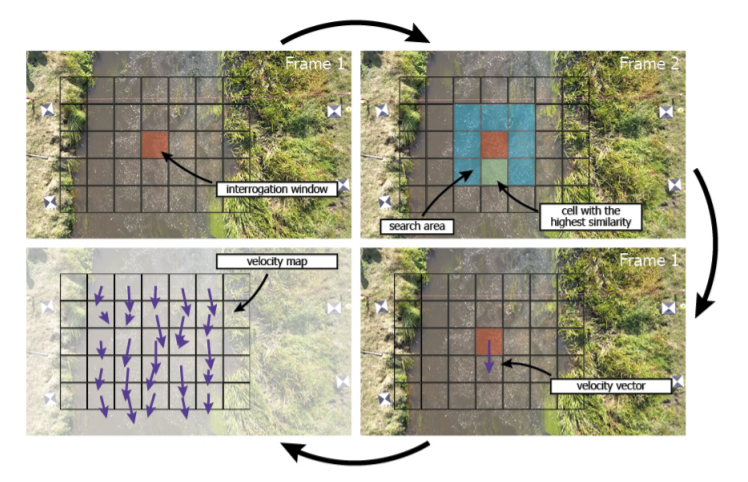
\includegraphics[width=1\linewidth,]{images/pivprocessing} \caption{Vue schématique de la méthode LSPIV où une fenêtre d'interrogation est déterminée (la grille est dessinée plus grande dan généralement appliqué) dans la première image et les graines présentes sont comparées à une zone de recherche dans l'image séquentielle 2 à déterminer leurs déplacements. En multipliant le déplacement par la période de temps de trame, la vitesse est déterminée. Lorsque vous appliquez ceci sur toute l'image, une carte de vitesse d'écoulement de surface peut être créée pour chaque image individuelle.}\label{fig:fpivprocessing}
\end{figure}

\begin{Shaded}
\begin{Highlighting}[]
\ImportTok{import}\NormalTok{ os}
\ImportTok{import}\NormalTok{ numpy }\ImportTok{as}\NormalTok{ np}
\ImportTok{import}\NormalTok{ pandas }\ImportTok{as}\NormalTok{ pd}
\ImportTok{from}\NormalTok{ tqdm }\ImportTok{import}\NormalTok{ tqdm}
\ImportTok{from}\NormalTok{ openpiv }\ImportTok{import}\NormalTok{ tools,pyprocess,validation, filters,scaling}
\ImportTok{import}\NormalTok{ matplotlib.pyplot }\ImportTok{as}\NormalTok{ plt}
\end{Highlighting}
\end{Shaded}

\begin{Shaded}
\begin{Highlighting}[]
\KeywordTok{def}\NormalTok{ PIV(}
\NormalTok{    frame\_0,}
\NormalTok{    frame\_1,}
\NormalTok{    winsize,}
\NormalTok{    searchsize,}
\NormalTok{    overlap,}
\NormalTok{    frame\_rate,}
\NormalTok{    scaling\_factor,}
\NormalTok{    threshold}\OperatorTok{=}\FloatTok{1.3}\NormalTok{,}
\NormalTok{    output}\OperatorTok{=}\StringTok{\textquotesingle{}fil\textquotesingle{}}\NormalTok{ ):}

    \CommentTok{\# déterminer le pas de temps entre les deux images séquentielles (1 / fps)}
\NormalTok{    dt }\OperatorTok{=} \FloatTok{1.}\OperatorTok{/}\NormalTok{frame\_rate}

    \CommentTok{\# estimation des déplacements de graines dans les directions x et y}
    \CommentTok{\# et le rapport signal / bruit correspondant}
\NormalTok{    u, v, sig2noise }\OperatorTok{=}\NormalTok{ pyprocess.extended\_search\_area\_piv(}
\NormalTok{                        frame\_a }\OperatorTok{=}\NormalTok{ frame\_0,}
\NormalTok{                        frame\_b }\OperatorTok{=}\NormalTok{ frame\_1,}
\NormalTok{                        window\_size }\OperatorTok{=}\NormalTok{ winsize,}
\NormalTok{                        overlap }\OperatorTok{=}\NormalTok{ overlap,}
\NormalTok{                        dt}\OperatorTok{=}\NormalTok{dt,}
\NormalTok{                        search\_area\_size }\OperatorTok{=}\NormalTok{ searchsize,      }
\NormalTok{                        sig2noise\_method }\OperatorTok{=} \StringTok{\textquotesingle{}peak2peak\textquotesingle{}}\NormalTok{)}

    \CommentTok{\# coordonnées xy du centre de chaque cellule de la grille}
\NormalTok{    x, y }\OperatorTok{=}\NormalTok{ pyprocess.get\_coordinates(image\_size}\OperatorTok{=}\NormalTok{frame\_0.shape,}
\NormalTok{                                     search\_area\_size}\OperatorTok{=}\NormalTok{winsize,}
\NormalTok{                                     overlap}\OperatorTok{=}\NormalTok{overlap)}

    \CommentTok{\# si la sortie est \textquotesingle{}fill\textquotesingle{} ou \textquotesingle{}int\textquotesingle{}:}
    \CommentTok{\# filtrer les cellules de la grille avec un faible rapport signal / bruit}
    \ControlFlowTok{if}\NormalTok{ output }\OperatorTok{==} \StringTok{\textquotesingle{}fil\textquotesingle{}} \KeywordTok{or}\NormalTok{  output }\OperatorTok{==} \StringTok{\textquotesingle{}int\textquotesingle{}}\NormalTok{:}
\NormalTok{        u, v, mask }\OperatorTok{=}\NormalTok{ validation.sig2noise\_val(u,}
\NormalTok{                                              v,}
\NormalTok{                                              sig2noise,}
\NormalTok{                                              threshold}\OperatorTok{=}\NormalTok{threshold)}

    \CommentTok{\# si la sortie est \textquotesingle{}int\textquotesingle{}}
    \CommentTok{\# remplir les valeurs manquantes par interpolation}
    \ControlFlowTok{if}\NormalTok{ output }\OperatorTok{==} \StringTok{\textquotesingle{}int\textquotesingle{}}\NormalTok{:}
\NormalTok{        u, v }\OperatorTok{=}\NormalTok{ filters.replace\_outliers(u,}
\NormalTok{                                        v,}
\NormalTok{                                        method}\OperatorTok{=}\StringTok{\textquotesingle{}localmean\textquotesingle{}}\NormalTok{,}
\NormalTok{                                        max\_iter}\OperatorTok{=}\DecValTok{50}\NormalTok{,}
\NormalTok{                                        kernel\_size}\OperatorTok{=}\DecValTok{3}\NormalTok{)}

    \CommentTok{\# mettre à l\textquotesingle{}échelle les résultats en fonction des pixels par mètre}
\NormalTok{    x, y, u, v }\OperatorTok{=}\NormalTok{ scaling.uniform(x,}
\NormalTok{                                 y,}
\NormalTok{                                 u,}
\NormalTok{                                 v,}
\NormalTok{                                 scaling\_factor}\OperatorTok{=}\NormalTok{scaling\_factor)}

    \ControlFlowTok{return}\NormalTok{ x, y, u, v, sig2noise}
\end{Highlighting}
\end{Shaded}

\begin{Shaded}
\begin{Highlighting}[]
\NormalTok{dir\_frames }\OperatorTok{=} \StringTok{\textquotesingle{}Python/frames\textquotesingle{}}
\NormalTok{dir\_saves }\OperatorTok{=} \StringTok{\textquotesingle{}Python/files\textquotesingle{}}

\ControlFlowTok{if} \KeywordTok{not}\NormalTok{ os.path.exists(dir\_saves):}
\NormalTok{    os.mkdir(dir\_saves)}
\end{Highlighting}
\end{Shaded}

\begin{Shaded}
\begin{Highlighting}[]
\NormalTok{winsize }\OperatorTok{=}  \DecValTok{60}            \CommentTok{\# pixels, taille de la fenêtre d\textquotesingle{}interrogation dans l\textquotesingle{}image A}
\NormalTok{searchsize }\OperatorTok{=}\NormalTok{ winsize     }\CommentTok{\# pixels, recherche dans l\textquotesingle{}image B}
\NormalTok{overlap }\OperatorTok{=}  \DecValTok{30}            \CommentTok{\# pixels, chevauchement de 50\%}
\NormalTok{frame\_rate }\OperatorTok{=} \DecValTok{25}          \CommentTok{\# vidéo à fréquence d\textquotesingle{}images}
\NormalTok{scaling\_factor }\OperatorTok{=} \DecValTok{100}     \CommentTok{\# pixels par mètre (PPM)}
\NormalTok{threshold }\OperatorTok{=} \FloatTok{1.3}          \CommentTok{\# rapport signal / bruit auquel les résultats sont filtrés}
\end{Highlighting}
\end{Shaded}

\begin{Shaded}
\begin{Highlighting}[]
\CommentTok{\# importer les noms et le nombre de cadres}
\NormalTok{frames }\OperatorTok{=}\NormalTok{ os.listdir(dir\_frames)}
\NormalTok{N }\OperatorTok{=} \BuiltInTok{len}\NormalTok{(frames)}\OperatorTok{{-}}\DecValTok{1}

\ControlFlowTok{for}\NormalTok{ n }\KeywordTok{in}\NormalTok{ tqdm(}\BuiltInTok{range}\NormalTok{(N)):}
    \CommentTok{\# définir les deux trames séquentielles utilisées pour estimer le champ de vitesse}
\NormalTok{    frame\_0 }\OperatorTok{=}\NormalTok{ tools.imread(os.path.join(dir\_frames,}\BuiltInTok{str}\NormalTok{(frames[n])))}
\NormalTok{    frame\_1 }\OperatorTok{=}\NormalTok{ tools.imread(os.path.join(dir\_frames,}\BuiltInTok{str}\NormalTok{(frames[n}\OperatorTok{+}\DecValTok{1}\NormalTok{])))}

    \CommentTok{\# Traitement PIV}
\NormalTok{    x, y, u, v, sig2noise }\OperatorTok{=}\NormalTok{ PIV(frame\_0, frame\_1, winsize, searchsize,}
\NormalTok{                                overlap, frame\_rate, scaling\_factor,}
\NormalTok{                                threshold, output}\OperatorTok{=}\StringTok{\textquotesingle{}fil\textquotesingle{}}\NormalTok{)}

    \CommentTok{\# enregistrer les résultats dans un fichier texte}
\NormalTok{    tools.save(x,}
\NormalTok{               y,}
\NormalTok{               u,}
\NormalTok{               v,}
\NormalTok{               sig2noise,}
\NormalTok{               os.path.join(dir\_saves, }\BuiltInTok{str}\NormalTok{(}\BuiltInTok{format}\NormalTok{(n).zfill(}\DecValTok{6}\NormalTok{))}\OperatorTok{+}\StringTok{\textquotesingle{}.txt\textquotesingle{}}\NormalTok{))}
\end{Highlighting}
\end{Shaded}

\hypertarget{ad}{%
\section*{l'analyse des donnée}\label{ad}}
\addcontentsline{toc}{section}{l'analyse des donnée}

Ce fichier traite deux étapes de post-traitement pour acquérir des vitesses d'écoulement de surface à une section transversale spécifique. Les étapes de post-traitement sont nommées filtrage et substitution . Les deux processus sont expliqués dans les sections suivantes. Pour ces étapes, plusieurs informations supplémentaires sont nécessaires à savoir:

\begin{itemize}
\item
  bathymétrie locale,
\item
  niveau d'eau,
\item
  paramètres de progression verticale des vitesses d'écoulement de surface.
\end{itemize}

Dans les sections à venir, traiter les sujets suivants: (1) les résultats non traités, (2) le filtrage des vitesses d'écoulement inférieures, et (3) la substitution des vitesses d'écoulement en cas de manque de graines.

\begin{Shaded}
\begin{Highlighting}[]
\ImportTok{import}\NormalTok{ os}
\ImportTok{import}\NormalTok{ numpy }\ImportTok{as}\NormalTok{ np}
\ImportTok{import}\NormalTok{ matplotlib.pyplot }\ImportTok{as}\NormalTok{ plt}
\ImportTok{import}\NormalTok{ pandas }\ImportTok{as}\NormalTok{ pd}
\ImportTok{from}\NormalTok{ scipy }\ImportTok{import}\NormalTok{ interpolate}
\end{Highlighting}
\end{Shaded}

\begin{Shaded}
\begin{Highlighting}[]
\NormalTok{dir\_files }\OperatorTok{=} \StringTok{\textquotesingle{}Python/files\textquotesingle{}}
\NormalTok{bat }\OperatorTok{=} \VerbatimStringTok{r\textquotesingle{}Python/bathymetry.csv\textquotesingle{}}
\end{Highlighting}
\end{Shaded}

\hypertarget{ruxe9sultats-non-traituxe9s}{%
\subsection*{Résultats non traités}\label{ruxe9sultats-non-traituxe9s}}
\addcontentsline{toc}{subsection}{Résultats non traités}

la zone d'intérêt se situe à 1 mètre à gauche et à trois mètres à droite du point central de la bathymétrie (fournie dans le fichier bathymetry.csv). Comme l'écoulement va de gauche à droite, seules les composantes x des vitesses d'écoulement sont utilisées pour estimer les vitesses d'écoulement moyennes.

La largeur du ruisseau est divisée en différentes sections transversales. Pour chaque section, les vitesses d'écoulement sont rassemblées et une valeur moyenne est déterminée.

Tout d'abord, certaines caractéristiques de base sont prouvées. L'emplacement du centre de la bathymétrie dans l'imagerie (\(centre_x\) et \(centre_y\)), les emplacements des berges du cours d'eau à la bathymétrie (\(y_0\) et \(y_1\)), et le niveau d'eau (\(w_l\)) pendant la vidéo.

\begin{Shaded}
\begin{Highlighting}[]
\CommentTok{\# localisation de la bathymétrie du centre dans l\textquotesingle{}imagerie (mètres).}
\CommentTok{\# Utilisé pour aligner les vitesses d\textquotesingle{}écoulement avec la bathymétrie}
\NormalTok{centre\_x, centre\_y }\OperatorTok{=}\NormalTok{ [}\FloatTok{8.3471579}\NormalTok{ , }\FloatTok{2.01868403}\NormalTok{]}

\CommentTok{\# emplacements banques de flux}
\NormalTok{y0, y1 }\OperatorTok{=}\NormalTok{ [}\OperatorTok{{-}}\FloatTok{1.397}\NormalTok{, }\FloatTok{3.785}\NormalTok{]}

\CommentTok{\# niveau d\textquotesingle{}eau (par rapport au point bathymétrique le plus bas)}
\NormalTok{wl }\OperatorTok{=} \FloatTok{0.9}
\end{Highlighting}
\end{Shaded}

La bathymétrie se trouve dans le fichier \textbf{bathymetry.csv}. Pour utiliser cette bathymétrie, les points sont interpolés à l'aide de la fonction scipy.interpolate.interpolate.

\begin{Shaded}
\begin{Highlighting}[]

\CommentTok{\# importer la bathymétrie locale}
\NormalTok{df\_bat }\OperatorTok{=}\NormalTok{ pd.read\_table(bat, sep}\OperatorTok{=}\StringTok{\textquotesingle{};\textquotesingle{}}\NormalTok{, usecols}\OperatorTok{=}\NormalTok{[}\StringTok{\textquotesingle{}Y\textquotesingle{}}\NormalTok{, }\StringTok{\textquotesingle{}H\textquotesingle{}}\NormalTok{])}
\CommentTok{\# fonction interpolée de la bathymétrie}
\NormalTok{func\_bat }\OperatorTok{=}\NormalTok{ interpolate.interp1d(df\_bat[}\StringTok{\textquotesingle{}Y\textquotesingle{}}\NormalTok{], df\_bat[}\StringTok{\textquotesingle{}H\textquotesingle{}}\NormalTok{], kind}\OperatorTok{=}\StringTok{\textquotesingle{}quadratic\textquotesingle{}}\NormalTok{)}


\NormalTok{plt.figure(figsize}\OperatorTok{=}\NormalTok{ (}\DecValTok{12}\NormalTok{,}\DecValTok{4}\NormalTok{))}
\NormalTok{plt.scatter(df\_bat.Y,df\_bat.H,alpha}\OperatorTok{=}\FloatTok{0.5}\NormalTok{,label }\OperatorTok{=}\StringTok{"Mesures individuelles"}\NormalTok{)}
\NormalTok{plt.plot(df\_bat.Y,func\_bat(df\_bat.Y),color }\OperatorTok{=}\StringTok{"black"}\NormalTok{, alpha}\OperatorTok{=}\FloatTok{0.3}\NormalTok{,label}\OperatorTok{=} \StringTok{"Bathymétrie interpolée"}\NormalTok{)}
\NormalTok{plt.xlabel(}\StringTok{\textquotesingle{}Y [m]\textquotesingle{}}\NormalTok{)}
\NormalTok{plt.ylabel(}\StringTok{\textquotesingle{}Z [m]\textquotesingle{}}\NormalTok{)}
\NormalTok{plt.legend(loc }\OperatorTok{=} \StringTok{\textquotesingle{}lower right\textquotesingle{}}\NormalTok{)}
\NormalTok{plt.show()}
\end{Highlighting}
\end{Shaded}

\begin{figure}[H]
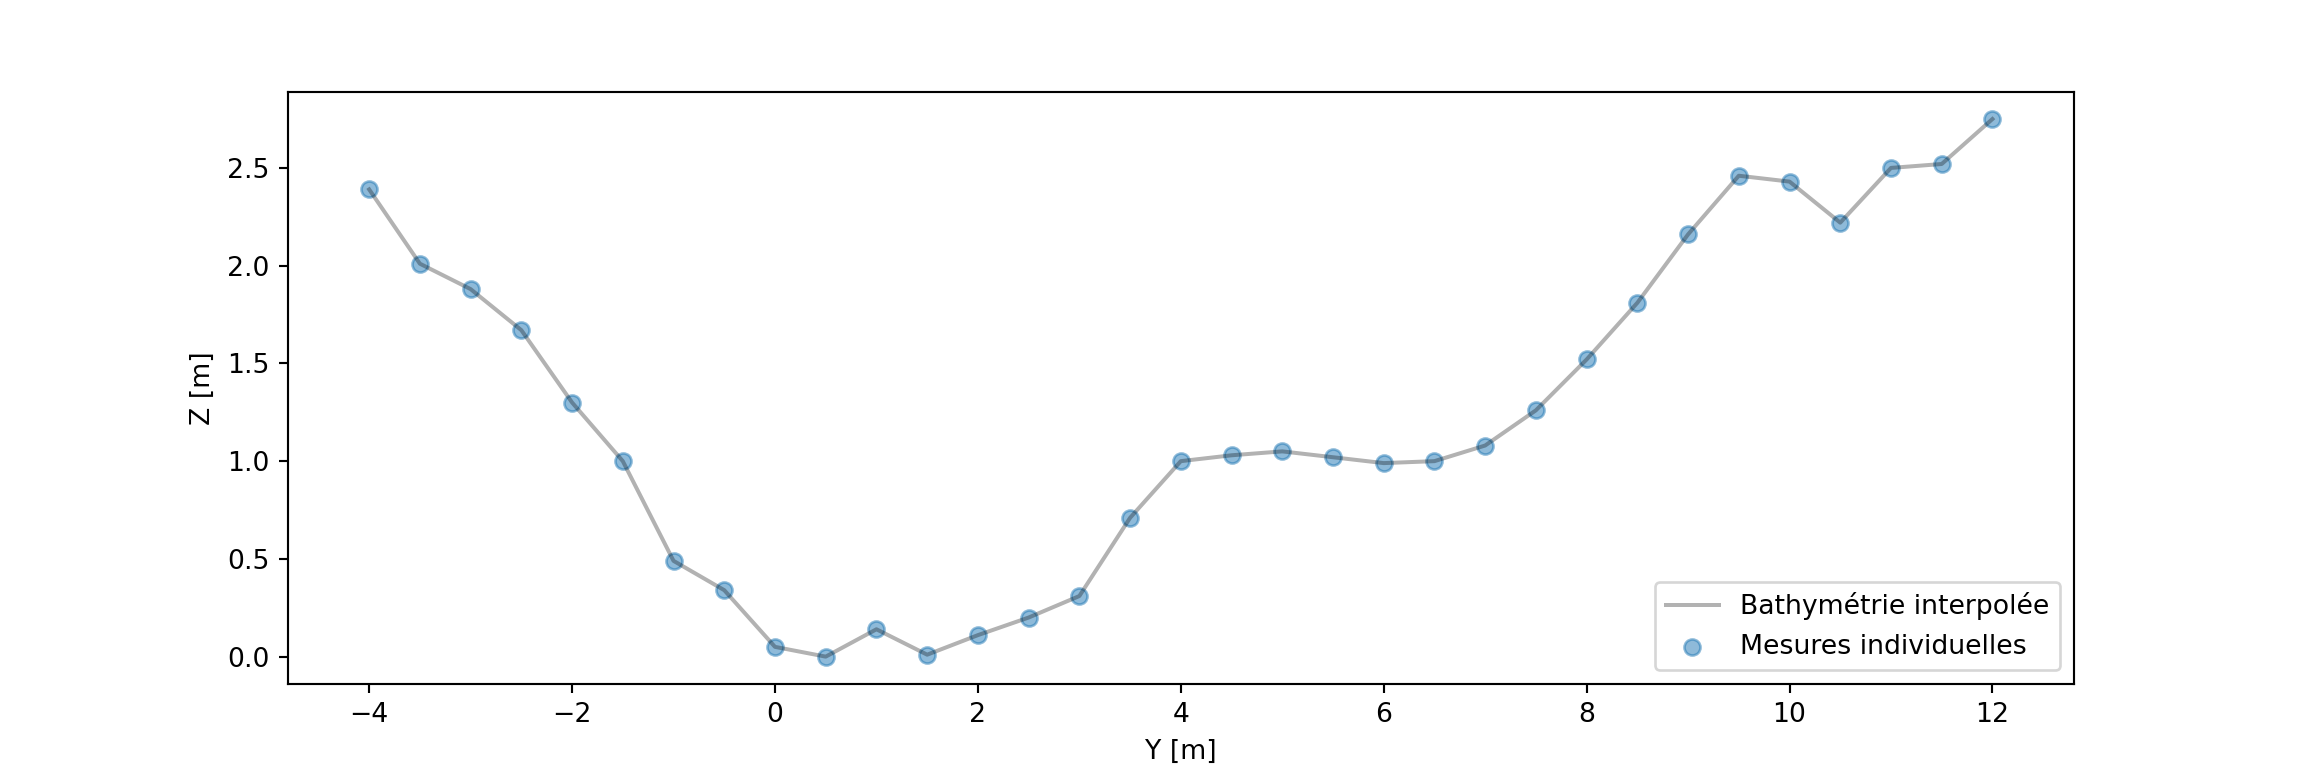
\includegraphics[width=1\linewidth,]{PROJET_LSPIV_files/figure-latex/unnamed-chunk-17-1} \caption{la bathymétrie locale}\label{fig:unnamed-chunk-17}
\end{figure}

\begin{Shaded}
\begin{Highlighting}[]
\CommentTok{\# extraire les noms des fichiers texte}
\NormalTok{files }\OperatorTok{=}\NormalTok{ os.listdir(dir\_files)}

\CommentTok{\# créer un dataframe dans lequel toutes les vitesses de la zone d\textquotesingle{}intérêt sont stockées}
\NormalTok{vx\_all }\OperatorTok{=}\NormalTok{ pd.DataFrame()}

\CommentTok{\# créer un tableau pour enregistrer les vitesses moyennes}
\NormalTok{vx\_mean\_raw }\OperatorTok{=}\NormalTok{ []}

\ControlFlowTok{for} \BuiltInTok{file} \KeywordTok{in}\NormalTok{ files:}
    \CommentTok{\# importer un fichier unique et ajouter des vitesses dans la zone d\textquotesingle{}intérêt}
    \CommentTok{\# à la trame de données}
\NormalTok{    df }\OperatorTok{=}\NormalTok{ pd.read\_table(os.path.join(dir\_files, }\BuiltInTok{file}\NormalTok{),}
\NormalTok{                       sep}\OperatorTok{=}\StringTok{\textquotesingle{}\textbackslash{}s+\textquotesingle{}}\NormalTok{,}
\NormalTok{                       names}\OperatorTok{=}\NormalTok{(}\StringTok{\textquotesingle{}X\textquotesingle{}}\NormalTok{, }\StringTok{\textquotesingle{}Y\textquotesingle{}}\NormalTok{, }\StringTok{\textquotesingle{}Vx\textquotesingle{}}\NormalTok{, }\StringTok{\textquotesingle{}Vy\textquotesingle{}}\NormalTok{, }\StringTok{\textquotesingle{}s2n\textquotesingle{}}\NormalTok{),}
\NormalTok{                       header}\OperatorTok{=}\DecValTok{0}\NormalTok{,}
\NormalTok{                       index\_col}\OperatorTok{=} \VariableTok{False}\NormalTok{)  }
\NormalTok{    df[}\StringTok{\textquotesingle{}X\textquotesingle{}}\NormalTok{]}\OperatorTok{=}\NormalTok{df[}\StringTok{\textquotesingle{}X\textquotesingle{}}\NormalTok{].astype(}\StringTok{\textquotesingle{}float\textquotesingle{}}\NormalTok{)}
\NormalTok{    df[}\StringTok{\textquotesingle{}Y\textquotesingle{}}\NormalTok{]}\OperatorTok{=}\NormalTok{df[}\StringTok{\textquotesingle{}Y\textquotesingle{}}\NormalTok{].astype(}\StringTok{\textquotesingle{}float\textquotesingle{}}\NormalTok{)}
\NormalTok{    df[}\StringTok{\textquotesingle{}Vx\textquotesingle{}}\NormalTok{]}\OperatorTok{=}\NormalTok{df[}\StringTok{\textquotesingle{}Vx\textquotesingle{}}\NormalTok{].astype(}\StringTok{\textquotesingle{}float\textquotesingle{}}\NormalTok{)}
\NormalTok{    df[}\StringTok{\textquotesingle{}Vy\textquotesingle{}}\NormalTok{]}\OperatorTok{=}\NormalTok{df[}\StringTok{\textquotesingle{}Vy\textquotesingle{}}\NormalTok{].astype(}\StringTok{\textquotesingle{}float\textquotesingle{}}\NormalTok{)}
\NormalTok{    df }\OperatorTok{=}\NormalTok{ df[df[}\StringTok{\textquotesingle{}X\textquotesingle{}}\NormalTok{] }\OperatorTok{\textgreater{}}\NormalTok{ (centre\_x }\OperatorTok{{-}} \DecValTok{1}\NormalTok{)]}
\NormalTok{    df }\OperatorTok{=}\NormalTok{ df[df[}\StringTok{\textquotesingle{}X\textquotesingle{}}\NormalTok{] }\OperatorTok{\textless{}}\NormalTok{ (centre\_x }\OperatorTok{+} \DecValTok{3}\NormalTok{)]}
\NormalTok{    vx\_all }\OperatorTok{=}\NormalTok{ vx\_all.append(df)}

\CommentTok{\# définir les différentes coordonnées y (sections de largeur de flux)}
\NormalTok{y\_unique }\OperatorTok{=}\NormalTok{ np.sort(df.Y.unique())}
    
\CommentTok{\# corriger les coordonnées y par rapport au \textquotesingle{}centre\textquotesingle{} bathymétrique}
\NormalTok{y\_corrected }\OperatorTok{=}\NormalTok{ y\_unique }\OperatorTok{{-}}\NormalTok{ centre\_y}
\end{Highlighting}
\end{Shaded}

\hypertarget{filtrage}{%
\subsection*{Filtrage}\label{filtrage}}
\addcontentsline{toc}{subsection}{Filtrage}

Comme la densité d'ensemencement n'est pas assez dense pour avoir des graines à chaque cellule de la grille, il y a des moments où aucune vitesse d'écoulement de surface n'est estimée, ce qui entraîne une large gamme de vitesses d'écoulement. Par conséquent, un filtrage supplémentaire est appliqué pour supprimer les estimations de vitesse d'écoulement inférieure.

Ce filtrage est basé sur la distance d'une mesure par rapport à la vitesse d'écoulement du 95e percentile dans cette section transversale. Si une valeur est plus éloignée que deux fois l'écart type du 95er centile, cette valeur est filtrée. Ou en bref, le filtrage est appliqué lorsque l'instruction suivante est remplie:

\begin{equation}
V_{X} < V_{q95} - 2 \cdot \sigma_{V_{X}}
\end{equation}

Comme cette déclaration peut entraîner un filtrage excessif, une autre instruction (ou seuil) doit être satisfaite avant que le filtrage ne soit appliqué à une section transversale. Le 95e centile doit être supérieur à 2,5 fois l'écart type:

\begin{equation}
V_{q95} > 2.5 \cdot \sigma_{V_{X}}
\end{equation}

Les nouvelles estimations des vitesses d'écoulement moyennes peuvent être faites.

\begin{Shaded}
\begin{Highlighting}[]
\CommentTok{\# tableau pour stocker les vitesses d\textquotesingle{}écoulement moyennes}
\NormalTok{vx\_mean\_fil }\OperatorTok{=}\NormalTok{ []}

\CommentTok{\# pour chaque section transversale}
\CommentTok{\# trouver les vitesses d\textquotesingle{}écoulement correspondantes et supprimer les valeurs NaN}
\ControlFlowTok{for}\NormalTok{ yy }\KeywordTok{in}\NormalTok{ y\_unique:}
\NormalTok{    vxi }\OperatorTok{=}\NormalTok{ vx\_all.Vx[vx\_all.Y }\OperatorTok{==}\NormalTok{ yy]}
\NormalTok{    vxi }\OperatorTok{=}\NormalTok{ vxi[np.isfinite(vxi)]}

    \CommentTok{\# si toutes les valeurs sont NaN, créez un tableau de longueur 1}
    \ControlFlowTok{if} \BuiltInTok{len}\NormalTok{(vxi) }\OperatorTok{==} \DecValTok{0}\NormalTok{:}
\NormalTok{        vxi }\OperatorTok{=}\NormalTok{ [}\DecValTok{0}\NormalTok{]}
    
    \CommentTok{\# déterminer le 95e quantile et l\textquotesingle{}écart type}
\NormalTok{    v\_filter }\OperatorTok{=}\NormalTok{ np.quantile(vxi, }\FloatTok{0.95}\NormalTok{)}
\NormalTok{    std }\OperatorTok{=}\NormalTok{ np.std(vxi)}

    \CommentTok{\# le filtrage est appliqué si le 95e centile\textgreater{} 2,5 * std}
    \ControlFlowTok{if} \FloatTok{2.5}\OperatorTok{*}\NormalTok{std}\OperatorTok{/}\NormalTok{v\_filter }\OperatorTok{\textless{}} \DecValTok{1}\NormalTok{:}
        \CommentTok{\# le filtrage est appliqué sur les valeurs plus éloignées que 2 * std du 95e centile}
\NormalTok{        vxi\_in }\OperatorTok{=}\NormalTok{ vxi[vxi }\OperatorTok{\textgreater{}}\NormalTok{ v\_filter }\OperatorTok{{-}} \DecValTok{2}\OperatorTok{*}\NormalTok{std]}
\NormalTok{        vxi\_out }\OperatorTok{=}\NormalTok{ vxi[vxi }\OperatorTok{\textless{}}\NormalTok{ v\_filter }\OperatorTok{{-}} \DecValTok{2}\OperatorTok{*}\NormalTok{std]}
        \CommentTok{\# ajouter une valeur moyenne en fonction des résultats filtrés}
\NormalTok{        vx\_mean\_fil.append(np.mean(vxi\_in))}

    \CommentTok{\# si le filtrage n\textquotesingle{}est pas appliqué: déterminer la moyenne sur toutes les valeurs}
    \ControlFlowTok{else}\NormalTok{:}
\NormalTok{      vx\_mean\_fil.append(np.mean(vxi))}
\end{Highlighting}
\end{Shaded}

\hypertarget{substitution}{%
\subsection*{Substitution}\label{substitution}}
\addcontentsline{toc}{subsection}{Substitution}

Comme dans certaines sections transversales aucune graine n'est présente, les vitesses d'écoulement sont à coup sûr sous-estimées à ces endroits. Pour encore faire une estimation éclairée des vitesses d'écoulement à ces endroits, les vitesses d'écoulement à différents stades de l'onde de crue sont estimées et utilisées pour établir une relation entre les vitesses d'écoulement de surface et la profondeur de l'eau. Cette relation est approchée en utilisant la loi logarithmique de Prandtl-von Kármán:

\begin{equation}
V_{x_sub}(h) = \frac{u_{\star}}{\kappa} \ln\left[\frac{h - d}{h_0}\right]
\end{equation}

Dans cette formule \(V_{x_sub}(h)\) est la vitesse d'écoulement à la profondeur de l'eau \(h\); \(u_{\star}\) est la vitesse de cisaillement;\(\kappa\) est la constante de von Kármán (\(\approx 0.41\)); \(h_0\) est la profondeur de rugosité; \(d\) est le déplacement dans le plan zéro. Pour l'exemple de vidéo, \(u_{\star}\) , \(h_0\) et \(d\) sont estimés à \(0.235\) , \(0.054\) et \(0.15\).

Les vitesses d'écoulement de surface sont remplacées si la vitesse d'écoulement de surface est la moitié de la valeur de substitution et lorsque la section se trouve dans les berges du cours d'eau.

\begin{Shaded}
\begin{Highlighting}[]
\KeywordTok{def}\NormalTok{ vertical\_flow(loc\_wd, p, d}\OperatorTok{=}\FloatTok{0.15}\NormalTok{):}
\NormalTok{    us }\OperatorTok{=}\NormalTok{ p[}\DecValTok{0}\NormalTok{]}
\NormalTok{    h0 }\OperatorTok{=}\NormalTok{ p[}\DecValTok{1}\NormalTok{]}
    \ControlFlowTok{return}\NormalTok{ us}\OperatorTok{/}\FloatTok{0.41} \OperatorTok{*}\NormalTok{ np.log((loc\_wd }\OperatorTok{{-}}\NormalTok{ d) }\OperatorTok{/}\NormalTok{ h0)}

\CommentTok{\# paramètres de vitesse d\textquotesingle{}écoulement de surface de progression verticale}
\NormalTok{param }\OperatorTok{=}\NormalTok{ [}\FloatTok{0.235}\NormalTok{, }\FloatTok{0.054}\NormalTok{]}
\end{Highlighting}
\end{Shaded}

\begin{Shaded}
\begin{Highlighting}[]
\CommentTok{\# créer une copie des vitesses d\textquotesingle{}écoulement moyennes filtrées}
\NormalTok{vx\_mean\_rep }\OperatorTok{=}\NormalTok{ vx\_mean\_fil.copy()}

\CommentTok{\# déterminer les profondeurs d\textquotesingle{}eau à différentes coordonnées y corrigées}
\CommentTok{\# s\textquotesingle{}il y a de l\textquotesingle{}eau (wd\textgreater{} 0) et si y est compris entre {-}3 et 3 (pas de buissons)}
\CommentTok{\# si moyenne * 2 \textless{}valeur trouvée en utilisant le profil vertical}
\NormalTok{wd }\OperatorTok{=}\NormalTok{ wl }\OperatorTok{{-}}\NormalTok{ func\_bat(y\_corrected)}
\ControlFlowTok{for}\NormalTok{ nn, loc\_wd }\KeywordTok{in} \BuiltInTok{enumerate}\NormalTok{(wd):}
    \ControlFlowTok{if}\NormalTok{ loc\_wd }\OperatorTok{\textgreater{}} \FloatTok{0.15}\NormalTok{:}
        \ControlFlowTok{if}\NormalTok{ (y\_corrected[nn] }\OperatorTok{\textgreater{}} \OperatorTok{{-}}\FloatTok{3.5}\NormalTok{) }\KeywordTok{and}\NormalTok{ y\_corrected[nn] }\OperatorTok{\textless{}} \FloatTok{3.5}\NormalTok{:}
            \CommentTok{\# si 2 * la valeur médiane est inférieure à la valeur corrigée: valeur correcte}
            \CommentTok{\# tous les centiles}
            \ControlFlowTok{if}\NormalTok{ vx\_mean\_rep[nn] }\OperatorTok{\textless{}} \FloatTok{0.5}\OperatorTok{*}\NormalTok{vertical\_flow(loc\_wd, param):}
\NormalTok{                    vx\_mean\_rep[nn] }\OperatorTok{=}\NormalTok{ vertical\_flow(loc\_wd, param)}
\end{Highlighting}
\end{Shaded}

\begin{Shaded}
\begin{Highlighting}[]
\CommentTok{\# afficher les vitesses individuelles et les vitesses moyennes des différentes étapes }
\CommentTok{\# de post{-}traitement}
\NormalTok{fig }\OperatorTok{=}\NormalTok{ plt.figure(figsize}\OperatorTok{=}\NormalTok{(}\DecValTok{6}\NormalTok{,}\DecValTok{9}\NormalTok{))}
\NormalTok{plt.plot(vx\_mean\_rep, y\_corrected,}
\NormalTok{         color}\OperatorTok{=}\StringTok{\textquotesingle{}darkred\textquotesingle{}}\NormalTok{, marker}\OperatorTok{=}\StringTok{\textquotesingle{}x\textquotesingle{}}\NormalTok{, zorder}\OperatorTok{=}\DecValTok{2}\NormalTok{, alpha}\OperatorTok{=}\FloatTok{0.75}\NormalTok{, label}\OperatorTok{=}\StringTok{\textquotesingle{}Substitué\textquotesingle{}}\NormalTok{)}
\NormalTok{plt.hlines([y0, y1], xmin}\OperatorTok{={-}}\FloatTok{0.35}\NormalTok{, xmax}\OperatorTok{=}\DecValTok{1}\NormalTok{, color}\OperatorTok{=}\StringTok{\textquotesingle{}k\textquotesingle{}}\NormalTok{, alpha}\OperatorTok{=}\FloatTok{0.3}\NormalTok{, label}\OperatorTok{=}\StringTok{\textquotesingle{}Berges\textquotesingle{}}\NormalTok{)}
\NormalTok{plt.title(}\StringTok{"Vitesses d\textquotesingle{}ecoulement et leurs valeurs moyennes"}\NormalTok{)}
\NormalTok{plt.xlabel(}\StringTok{\textquotesingle{}Vx [m/s]\textquotesingle{}}\NormalTok{)}
\NormalTok{plt.ylabel(}\StringTok{\textquotesingle{}largeur du flux [m]\textquotesingle{}}\NormalTok{)}
\NormalTok{plt.xlim(}\OperatorTok{{-}}\FloatTok{.5}\NormalTok{, }\DecValTok{3}\NormalTok{)}
\end{Highlighting}
\end{Shaded}

\begin{verbatim}
## (-0.5, 3.0)
\end{verbatim}

\begin{Shaded}
\begin{Highlighting}[]
\NormalTok{plt.legend()}
\NormalTok{plt.show()}
\end{Highlighting}
\end{Shaded}

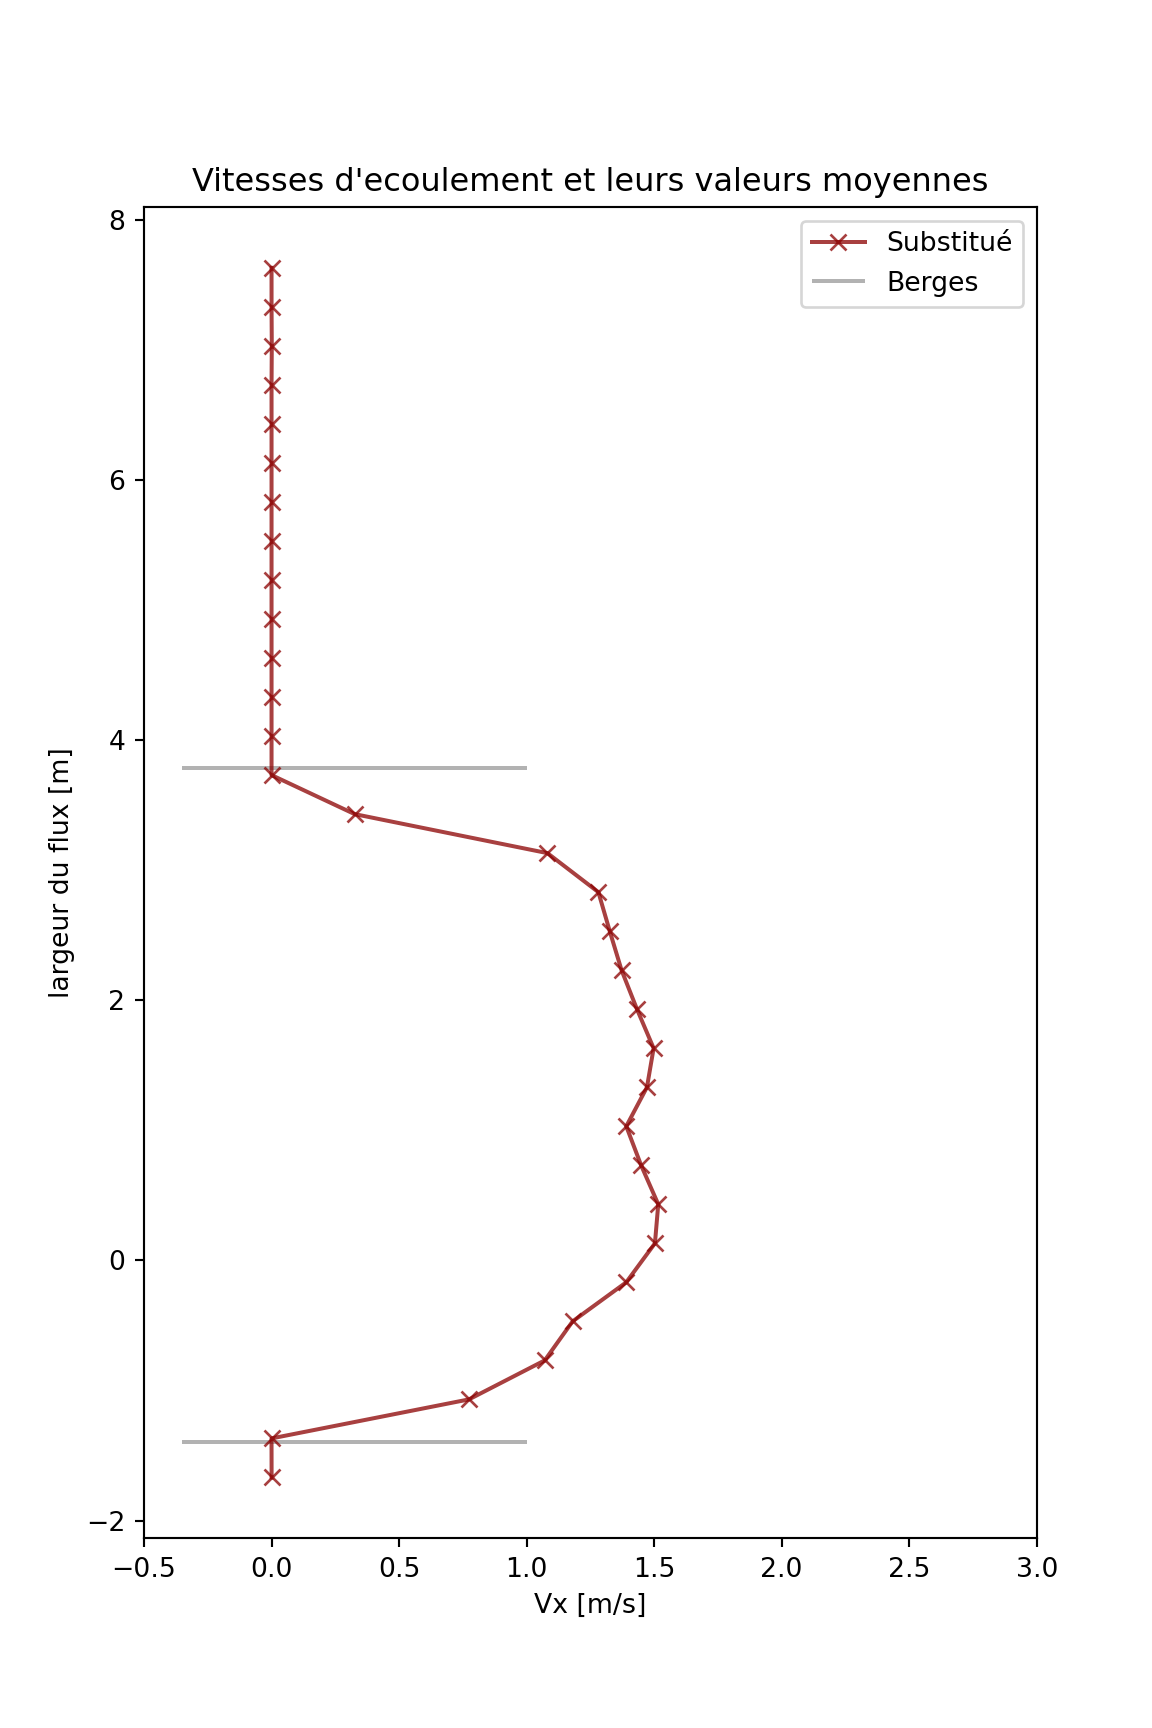
\includegraphics{PROJET_LSPIV_files/figure-latex/unnamed-chunk-22-1}

\hypertarget{estimation-de-duxe9charge}{%
\subsection*{Estimation de décharge}\label{estimation-de-duxe9charge}}
\addcontentsline{toc}{subsection}{Estimation de décharge}

Les rejets sont estimés en utilisant la méthode de la surface de vitesse, en utilisant la formule suivante:

\begin{equation}
Q = \sum_{n=1}^{N} v_n \cdot d_n \cdot b_n
\end{equation}

D'où \(v_n\) , \(d_n\), et \(b_n\) sont respectivement la vitesse d'écoulement, la profondeur et la largeur moyennes en profondeur de la section.

Pour la vitesse d'écoulement moyenne en profondeur, la vitesse d'écoulement de surface est multipliée par un coefficient déterminé empiriquement \(\alpha\). Ce coefficient est généralement entre \(0.72\) et \(0.95\). Pour l'exemple de vidéo, le coefficient est estimé à
\(0.85\).

\begin{Shaded}
\begin{Highlighting}[]
\CommentTok{\# coefficient moyen en profondeur}
\NormalTok{alpha }\OperatorTok{=} \FloatTok{0.85}

\CommentTok{\# sections transversales en largeur}
\NormalTok{step }\OperatorTok{=}\NormalTok{ y\_corrected[}\DecValTok{1}\NormalTok{]}\OperatorTok{{-}}\NormalTok{y\_corrected[}\DecValTok{0}\NormalTok{]}

\CommentTok{\# estimation de débit}
\NormalTok{Q }\OperatorTok{=} \BuiltInTok{sum}\NormalTok{(vx\_mean\_rep }\OperatorTok{*}\NormalTok{ wd  }\OperatorTok{*}\NormalTok{ alpha }\OperatorTok{*}\NormalTok{ step)}

\BuiltInTok{print}\NormalTok{(}\StringTok{"Le débit moyen est estimé à }\SpecialCharTok{\{\}}\StringTok{ m³/s"}\NormalTok{.}\BuiltInTok{format}\NormalTok{(}\BuiltInTok{round}\NormalTok{(Q, }\DecValTok{2}\NormalTok{)))}
\end{Highlighting}
\end{Shaded}

\begin{verbatim}
## Le débit moyen est estimé à 3.74 m³/s
\end{verbatim}

\newpage

  \bibliography{LSPIV.bib}

\end{document}
